\documentclass{report}

\usepackage{amsmath}
\usepackage{amsfonts}
\usepackage{amsthm}

\theoremstyle{plain}
\newtheorem{thm}{Theorem}[section]
\newtheorem{lem}[thm]{Lemma}
\newtheorem{prop}[thm]{Proposition}
\newtheorem*{cor}{Corollary}

\theoremstyle{definition}
\newtheorem{defn}{Definition}[section]
\newtheorem{conj}{Conjecture}[section]
\newtheorem{exmp}{Example}[section]

\theoremstyle{remark}
\newtheorem*{rem}{Remark}
\newtheorem*{note}{Note}

\usepackage{systeme}

\usepackage[T1]{fontenc}
\usepackage{dsfont}

\usepackage[top=2.5cm, left=3cm, right=3cm, bottom=2.5cm]{geometry}
\usepackage[demo]{graphicx}
\usepackage{caption}
\usepackage{subcaption}

\usepackage{etoolbox}
\listadd{\pc}{$C$}
\listadd{\pc}{$C\sharp$}
\listadd{\pc}{$D$}
\listadd{\pc}{$E\flat$}
\listadd{\pc}{$E$}
\listadd{\pc}{$F$}
\listadd{\pc}{$F\sharp$}
\listadd{\pc}{$G$}
\listadd{\pc}{$G\sharp$}
\listadd{\pc}{$A$}
\listadd{\pc}{$B\flat$}
\listadd{\pc}{$B$}
\listadd{\pcs}{$B$}
\listadd{\pcs}{$C$}
\listadd{\pcs}{$C\sharp$}
\listadd{\pcs}{$D$}
\listadd{\pcs}{$E\flat$}
\listadd{\pcs}{$E$}
\listadd{\pcs}{$F$}
\listadd{\pcs}{$F\sharp$}
\listadd{\pcs}{$G$}
\listadd{\pcs}{$G\sharp$}
\listadd{\pcs}{$A$}
\listadd{\pcs}{$B\flat$}

\usepackage{calc}

%\usepackage[pageanchor]{hyperref}
\captionsetup{margin=10pt,font=small,labelfont=bf}

\usepackage{tikz}
\usetikzlibrary{arrows,decorations.markings}
\usetikzlibrary{cd}
\usetikzlibrary{shapes.geometric,fit}
\usepackage{floatrow}
\newenvironment{tzfigure}[1]
{
    \begin{figure}[h]
        \centering
        #1
        \begin{tikzpicture}
}
{
        \end{tikzpicture}   
    \end{figure}
}

\newenvironment{tzcategory}[1]
{
    \begin{figure}[h]
        \centering
        #1
        \begin{tikzpicture}[baseline= (a).base]    
}
{
    \end{tikzpicture}   
\end{figure}
}


\usepackage{ stmaryrd }
\newcommand{\prodmon}{\Pi}
\usepackage{mathtools}
\newcommand{\phieq}{\stackrel{\mathclap{\normalfont\mbox{$\phi$}}}{\cong}}

\usepackage[refpage]{nomencl}
\makeatletter
\def\nomlabelref#1{\dotfill\nobreakspace page\ \pageref{#1}\nomentryend\endgroup}
\def\@@@nomenclature[#1]#2#3#4{%
 \def\@tempa{#2}\def\@tempb{#3}\def\@tempc{#4}%
 \protected@write\@nomenclaturefile{}%
  {\string\nomenclatureentry{#1\nom@verb\@tempa @[{\nom@verb\@tempa}]%
      \begingroup\nom@verb\@tempb\protect\nomeqref{\theequation}%
        |nomlabelref}{\@tempc}}%
 \endgroup
 \@esphack}
\makeatother
\usepackage[backref=page,pageanchor]{hyperref}
\renewcommand{\nomname}{Notations}
\renewcommand{\nompreamble}{The next list describes several notations used throughout this document.}
\makenomenclature



\begin{document}

%\begingroup    

\title{Categories and music}
\author{Alice Rixte}
\date{\today}
\maketitle %\endgroup
\nomenclature[010]{$[a,b]$}{Homset of all arrows between the object $a$ to the object $b$}{nomencl:Homset}
\nomenclature[020]{$\mathcal{C}/c$}{Slice category of $\mathcal{C}$ on the object $c$}{nomencl:slice}
\nomenclature[021]{$c/\mathcal{C}$}{Coslice category of $\mathcal{C}$ on the object $c$}{nomencl:coslice}
\nomenclature[022]{$\mathcal{C}\nnearrow c$}{Lax slice category of $\mathcal{C}$ on the object $c$}{nomencl:lax-slice}
\nomenclature[023]{$c\nnearrow\mathcal{C}$}{Lax coslice category of $\mathcal{C}$ on the object $c$}{nomencl:lax-coslice}
\nomenclature[024]{$\mathcal{C}\sswarrow c$}{Op-lax slice category of $\mathcal{C}$ on the object $c$}{nomencl:oplax-slice}
\nomenclature[025]{$c\sswarrow\mathcal{C}$}{Op-ax coslice category of $\mathcal{C}$ on the object $c$}{nomencl:oplax-coslice}
\nomenclature[026]{$\mathcal{C}/^s c$}{Strict slice category of $\mathcal{C}$ on the object $c$}{nomencl:strict-slice}
\nomenclature[027]{$c/^s\mathcal{C}$}{Strict coslice category of $\mathcal{C}$ on the object $c$}{nomencl:strict-coslice}
\nomenclature[Aut]{$Aut(G)$}{Automorphism group of $G$}{nomencl:Aut}
\nomenclature[Cat]{$\bf Cat$}{Category of small categories}{nomencl:Cat}
\nomenclature[CAT]{$\bf CAT$}{Category of locally small categories}{nomencl:CAT}
\nomenclature[EKN]{$\text{EKN}_{\mathcal{C}}$}{Category of EK-nets on the category $\mathcal{C}$}{nomencl:EKN}
\nomenclature[Ii]{$I_i$}{$i^\text{th}$ inversion}{nomencl:Ii}
\nomenclature[PKNR]{$\text{PKN}_R$}{Category of PK-nets of form $R$}{nomencl:PKNR}
\nomenclature[Set]{$\bf Set$}{Category of sets}{nomencl:Set}
\nomenclature[star]{$*$}{The category with one element and its identity arrow}{nomencl:star}
\nomenclature[TI]{$T/I$}{Group of transpositions and inversions acting on the set of pitch classes}	{nomencl:TI}
\nomenclature[Ti]{$T_i$}{Transposition of $i$ semitones}{nomencl:Ti}
\nomenclature[Zn]{$\mathbb{Z}_n$}{Cyclic group of order $n$}{nomencl:Zn}



\tableofcontents




\chapter{Introduction}
Transformational music theory is a way to analyse music by focusing on the transformations between musical object rather than on the objects themselves. It was mainly developped by David Lewins in 1980's \cite{rahn_lewin_1987}. His work relied on algebra, and particularly on group theory. Indeed, by using well temperament, we obtain a 12 element dodecahedron, with each vertex corresponding to one of the 12 semi-tones. Each vertex of this dodecahedron is called a \textbf{pitch class}(see Figure\ref{fig:dode-id}).

There are then 12 rotational symmetries and 12 axial symmetries of this dodecahedron (called  respectively \textbf{transpositions} and \textbf{inversions} and written $T_i$\label{nomencl:Ti} (see Figure \ref{fig:dode-T2}) and $I_i$\label{nomencl:Ii} (see Figure \ref{fig:dode-I4}) for $i\in [\![1,12]\!]$ by music theorists). If we only consider the transpositions, we actually a group isomorphic to the group $\mathbb{Z}_{12}$\label{nomencl:Zn}. The group composed of composed of the transpositions and the inversions is well known by mathematicians as the dihedral group but called by musicologists
$T/I$ \label{nomencl:TI} (see Figure \ref{fig:dode-TI}).

\begin{figure}[ht]
    \begin{subfigure}{.29\textwidth}
        \centering
        \newcounter{itemcount}
        \setcounter{itemcount}{450}
        \renewcommand*{\do}[1]{
            \filldraw [black](\number\value{itemcount}:3cm)
            circle (1.5pt)
            node[anchor={\number\value{itemcount}-180}]
                {#1\addtocounter{itemcount}{-30}};}
        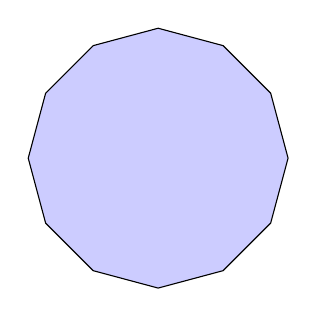
\begin{tikzpicture}[scale=0.55]
            \dolistloop{\pc}
            \draw[fill=blue!20] (90:3cm) -- (60:3cm) -- (30:3cm) -- (0:3cm) --  (330:3cm) -- (300:3cm) -- (270:3cm) -- (240:3cm) -- (210:3cm) -- (180 :3cm) -- (150:3cm) -- (120:3cm) -- cycle;
        \end{tikzpicture}
        \caption{The 12 pitch-classes dodecahedron}
        \label{fig:dode-id}
    \end{subfigure}%
    {\LARGE$\xRightarrow{T_2}$}%
    \begin{subfigure}{.3\textwidth}
        \centering
        \setcounter{itemcount}{510}
        \renewcommand*{\do}[1]{
            \filldraw [black](\number\value{itemcount}:3cm)
            circle (1.5pt)
            node[anchor={\number\value{itemcount}-180}]
                {#1\addtocounter{itemcount}{-30}};}
        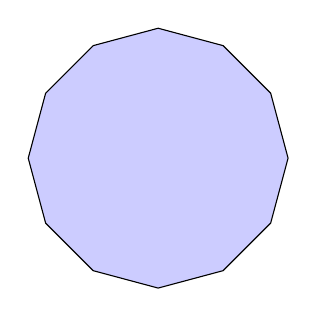
\begin{tikzpicture}[scale=0.55]
            \dolistloop{\pc}
            \draw[fill=blue!20] (90:3cm) -- (60:3cm) -- (30:3cm) -- (0:3cm) --  (330:3cm) -- (300:3cm) -- (270:3cm) -- (240:3cm) -- (210:3cm) -- (180 :3cm) -- (150:3cm) -- (120:3cm) -- cycle;
        \end{tikzpicture}
        \caption{Transposition of 2 semi-tones (Rotation)}
        \label{fig:dode-T2}
    \end{subfigure}%
    {\LARGE$\xRightarrow{I_4}$}%
    \begin{subfigure}{.3\textwidth}
        \centering
        \setcounter{itemcount}{510}
        \renewcommand*{\do}[1]{
            \filldraw [black](\number\value{itemcount}:3cm)
            circle (1.5pt)
            node[anchor={\number\value{itemcount}-180}]
                {#1\addtocounter{itemcount}{30}};}
        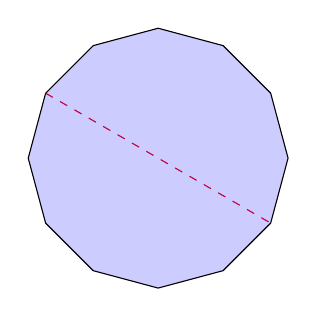
\begin{tikzpicture}[scale=0.55]

            \dolistloop{\pc}
            \draw[fill=blue!20] (90:3cm) -- (60:3cm) -- (30:3cm) -- (0:3cm) --  (330:3cm) -- (300:3cm) -- (270:3cm) -- (240:3cm) -- (210:3cm) -- (180 :3cm) -- (150:3cm) -- (120:3cm) -- cycle;
            \draw[purple,dashed] (150:3cm) -- (330:3cm);
        \end{tikzpicture}
        \caption{$4^{th}$ inversion  (Symmetry)}
        \label{fig:dode-I4}
    \end{subfigure}%
    \caption{Transpositions and inversions in a dodecahedron}
    \label{fig:dode-TI}
\end{figure}


This $T/I$ paradigm could then be applied to musical object. Indeed, we can represent a C major chord (see Figure \ref{fig:Cmajor}) inside the dodecahedron (to make the figure more readable, we changed the dodecahedron into a circle).
\newcounter{itemcount2}
\setcounter{itemcount2}{450}
\renewcommand*{\do}[1]{
    \filldraw [black](\number\value{itemcount2}:3cm)
    circle (1.5pt)
    node[anchor={\number\value{itemcount2}-180}]
        {#1\addtocounter{itemcount2}{-30}};}

\begin{tzfigure}{
        \caption{The C Major chord in the chromatic circle}
        \label{fig:Cmajor}
    }
    \dolistloop{\pc}
    \draw[fill=blue!20] (90:3cm) -- (330:3cm) -- (240:3cm) -- cycle;
    \draw [domain=0:360,samples=60] plot ({3*cos(\x)}, {3*sin(\x)});
\end{tzfigure}




% The intuition of Allen Forte was that instead of considering triads (three notes chord) as the set of the notes that compose them, we should consider them as the set of the intervals between each note. As a result, every inversion of chord \footnote{the term inversion has to be taken here from a musical point of view, for instance the inversions of a C major chord are C-E-G, G-C-E, E-G-C. Later in this report, we will use inversion as a member of the $T/I$ group and we will stick to it} will be in the same \textbf{pitch-class set}\cite{forte_1980}. This can be seen in the geometrical point of view where the simple fact  of representing the chord as a triangle allow to forget any order between the three note. Similarly, all the transpositions of the chord will be in the same pitch-class.


\section{Presentation of Klumpenhouwer's networks}
Klumpenhouwer networks, or K-nets, were then introduced by Henry Klumpenhouwer, former PhD student of Lewin, to formalize the relation between two chords\cite{lewin_1990}.

The idea behind K-nets is that instead of analyse chords transformations threw transposition only, which is not very rich, we could use also inversions.

\begin{defn}
    A Klumpenhouwer network is a graph (also called a network) where objects are pitch classes and arrows between objects are labeled by an element of the group $T/I$.
\end{defn}

\begin{defn}
    Two K-nets $K$ and $K'$ are said \textbf{isographic} if and only if :
    \begin{itemize}
        \item there exist a bijection $f:V(K)\rightarrow V(K')$ from the set of vertices $V(K)$ to $V(K')$
        \item if there is an arrow $a:s\rightarrow t$ where $s,t\in V(K)$ in $K$, then there is an arrow $a':f(s)\rightarrow f(t)$ in $K'$
        \item there is an automorphism $F \in Aut(T/I)$\label{nomencl:Aut} such that if $X$ is the label of an arrow $a:s\rightarrow t$, then $F(X)$ is the label of the arrow $a':f(s)\rightarrow f(t)$.
    \end{itemize}
\end{defn}

\begin{prop}[\cite{lewin_1990}]
    The T/I automorphisms are exactly the $F\big<u,j\big>$ such that $u\in\{1,5,7,11\}$ and $j\in\mathbb{Z}_{12}$ where
    \begin{align*}
        F\big<u,j\big>(T_n) & = T_{un}   \\
        F\big<u,j\big>(I_n) & = I_{un+j}
    \end{align*}
\end{prop}


\begin{note}
    The T/I automorphisms such that $u = 1$ (resp. $u = 11$) are called \textbf{positive automorphisms} (resp. \textbf{negative automorphisms}).
\end{note}


\begin{exmp}
    To represent a triad, Klumpenhouwer uses 3 pitch classes and 3 arrows of the form we can see in Figure \ref{fig:KCmajor}.
    Geometrically, we can see in Figure \ref{fig:Rtransf} that the inversion $I_4$ would transform our C major triangle into a A minor triangle (we swap C and E and G becomes A).
    \begin{tzfigure}{
            \caption{The $I_4$ inversion on the C major chord}
            \label{fig:Rtransf}
        }
        \dolistloop{\pc}
        \draw[fill=purple!20,opacity=0.7] (90:3cm) -- (330:3cm) -- (180:3cm) -- cycle;
        \draw[fill=blue!55, fill opacity=0.6] (90:3cm) -- (330:3cm) -- (240:3cm) -- cycle;
        \draw (90:3cm) -- (330:3cm) -- (240:3cm) -- cycle;
        \draw [dashed, thick, purple, opacity=1] (30:3cm) -- (210:3cm);
        \draw [domain=0:360,samples=60] plot ({3*cos(\x)}, {3*sin(\x)});
    \end{tzfigure}

    Actually, positive (resp. negative) isographies and transposition  (resp. inversions) are in one to one correspondance :
    \begin{align*}
        T_j & \mapsto F(1,j)  \\
        I_j & \mapsto F(11,j) \\
    \end{align*}
    This correspondance might seem hazardous but we will see that in EK-paradigm it is extremely accurate. If we follow this corresponence, we get an isography between two K-nets representing respectively C major and A minor (see Figure \ref{fig:Kisography}).
    \begin{figure}[h]

        \begin{subfigure}{.29\textwidth}
            \centering            
            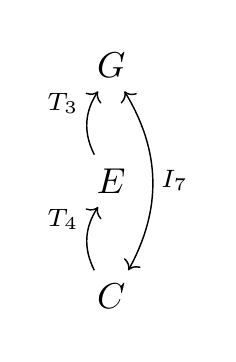
\begin{tikzpicture}
                % https://tikzcd.yichuanshen.de/#N4Igdg9gJgpgziAXAbVABwnAlgFyxMJZABgBoAmAXVJADcBDAGwFcYkQBhEAX1PU1z5CKMgEZqdJq3YBRHnxAZseAkTLEJDFm0QgA4jwkwoAc3hFQAMwBOEALZIyIHBCSiaAIxhgoSAMxOWtK6ACoA+gAs8la2Dojuzq6I5J7evogBNEE6IOF+0SA29o40LkgpIF4+SAC0mc70WIzskGBsNHAAFliWOCUgjPRejAAKAirCINZYJp19WVI5AJJhAOyG3EA
                \node[scale=1.3] (a) at (0,0){
                \begin{tikzcd}
                    G                                                            \\
                    E \arrow[u, "T_3", bend left]                                \\
                    C \arrow[u, "T_4", bend left] \arrow[uu, "I_7"',leftrightarrow,  bend right]
                \end{tikzcd}
                };
            \end{tikzpicture}
                        \caption{A Klumpenhouwer network for the C major chord}
            \label{fig:KCmajor}
        \end{subfigure}%
        {\LARGE$\xRightarrow{F\big<11,4\big>}$}%
        \begin{subfigure}{.29\textwidth}
            \centering
           
            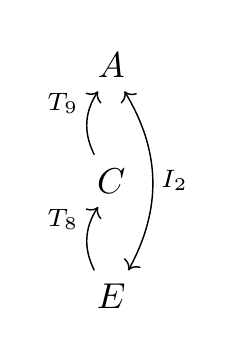
\begin{tikzpicture}

                % https://tikzcd.yichuanshen.de/#N4Igdg9gJgpgziAXAbVABwnAlgFyxMJZABgBoAmAXVJADcBDAGwFcYkQBhEAX1PU1z5CKMgEZqdJq3YBRHnxAZseAkTLEJDFm0QgA4jwkwoAc3hFQAMwBOEALZIyIHBCSiaAIxhgoSAMxOWtK6ACoA+gAs8la2Dojuzq6I5J7evogBNEE6IOF+0SA29o40LkgpIF4+SAC0mc70WIzskGBsNHAAFliWOCUgjPRejAAKAirCINZYJp19WVI5AJJhAOyG3EA
                \node[scale=1.3] (a) at (0,0){
                \begin{tikzcd}
                    A                                                            \\
                    C \arrow[u, "T_9", bend left]                                \\
                    E \arrow[u, "T_8", bend left] \arrow[uu, "I_2"',leftrightarrow,  bend right]
                \end{tikzcd}
                };
            \end{tikzpicture}
            \caption{A Klumpenhouwer network for A minor chord}
            \label{fig:KAminor}
        \end{subfigure}
        \caption{C major and A minor are isogrphic}
        \label{fig:Kisography}
    \end{figure}
\end{exmp}




\section{Presentation of PK-nets}
Klumpenhouwer networks propose many ways to analyse music but they do not allow to compare graphs of different form : if we want to compare a 3-note and a 4-note chord, there is no way there is an isography between K-nets representing them.

PK-nets\cite{PAAE2016} where introduced by Alexandre Popoff in 2015\cite{popoff2015categorical} and are a generalization of K-nets that allows comparison between any type of objects. They are defined in the paradigm of category theory. Let's first present informally category theory.

A category is a particular case of multigraph (i.e. a graph where there can be multiple arrows between to vertices), which means we are not so far from Klumpenhouwer's concept. However, one of the main goal of representing threw mathematics is to point some patterns or ways of construction usually used in music creation. So we would like to have a general enough mathematic construction so it encompasses as many musical concepts possible but restricted enough so that we are not overwhelmed by too many possible interpretation of the same piece of music.

In fact categories are one of the best framework to get a structured system without losing too many generalities.
One of the more important concept behind category theory is compositionality. Musically, it also seems a basic concept : if I can go from $C$ to $D$ and from $D$ to $E$, I would expect I can go from $C$ to $E$. This is in fact the whole concept of a scale : if from $C$, I can hit $D$, $E$, $F$, $G$, $A$, $B$ and finally to $C$ again, then, implicitely, I can go from any of the pitchs of the scale to another pitch of the scale.

A category is in fact a graph such that the composition of two arrows always exists and that for each vertex (called an object in category theory), there is an arrow on itself called the identity of this object. This is a minimal structure that we want to use to go further than the K-net analysis.

\begin{defn}\textbf{Set}\label{nomencl:Set} is the category where objects are the sets and morphisms are functions between sets.
\end{defn}

This is a non trivial definition, because we could face the Russell paradox. We will not go deeper in size problems in category. We will just point at the fact that we might have problem of size at some points.


The idea behind PK-nets is to lean on the category $\bf Set$ in such a way that musical objects are sets and relation between them are arrows. However, we need to add a frame to this principle. First of all, if we use the example of K-nets, we would like to use the group T/I to act on a 12 elements set. In fact, a group can be defined as a single-object category where the elements of the group are the reflexive arrows of this object and the group operation corresponds to the composition of two arrows.

The group action can be defined as a functor between the category T/I and the category $\bf Set$ which associates the unique object of T/I to a 12 elements set and the arrows to functions on this set. Indeed, functors in category theory are defined in such a way that they preserve identity and compositions, which makes every functor from a group to $\bf Set$ an action of this group on some set. So we have defined the set of pitch classes and how we want to analyse it.

We still need to know how to select some sets to be musical objects to analyse. For this, we use a category $\Delta$ where every object of $\Delta$ represents a musical object and the arrows between them their interactions. We then send  $\Delta$ on $\bf Set$ via a functor $R$ to have knowledge about the components of each musical object. But these interactions between objects are not defined either. So we need also a functor $F$ from $\Delta$ to $T/I$ which will exhibit how musical objects are related to each other.

To finish, we need to send each musical object seen as a set to the set of pitch-classes. This is the role of the natural transformation $\phi$. More formally,  as


\begin{defn}[PK-net\cite{popoff2015categorical}]
    \label{def:pk-net}
    For any category $\mathcal{C}$ and any functor $S:\mathcal{C} \rightarrow \Delta$ with non empty values (i.e. $\forall c \in \mathcal{C}, S(c) \neq \emptyset$), we can define a PK-net as follow :

    Let $\Delta$ be a small category and $R : \Delta \rightarrow \bf Set$ a functor with non empty values. Then a \textbf{PK-net} of form $R$ and with support $S$ is a tuple $\big<R,S,F,\phi\big>$ where $\phi : R \rightarrow SF$ is a natural transformation from $R$ to $SF$ (see Figure\ref{fig:PK-definition})

    \begin{tzcategory}{\caption{PK-net definition}
            \label{fig:PK-definition}}
        \node[scale=1.3] (a) at (0,0){
            \begin{tikzcd}[column sep=tiny]
                \Delta
                \ar[ddr, "R"',""{name=R,right}]
                \ar[rr,"F"]
                & &
                \mathcal{C}
                \ar[ddl,"S",""{name=S,left}] \\
                & \ar[Rightarrow,bend left=80,from=R, to=S, "\phi"']& \\
                & \bf Set &
            \end{tikzcd}
        };
    \end{tzcategory}

\end{defn}

As in the K-nets definition, we would like to transform a PK-net into another. However, we are forced here to have composition between homographies, since we are in a categorical paradigm.


\begin{defn}[Category of PK-nets\cite{popoff2015categorical}]
    For a fixed functor $R: \Delta \rightarrow \bf Set$, we can define the category $ \text{PKN}_R$ of PK-nets of form $R$ such that :
    \begin{itemize}
        \item the objects of $\text{PKN}_R$\label{nomencl:PKNR} are the PK-nets $\big<R,S,F,\phi\big>$ as defined in Definition \ref{def:pk-net}
        \item the morphisms between $\big<R,S,F,\phi\big>$ and $\big<R,S',F',\phi'\big>$ are pairs $\big< N,\nu\big>$ such that $N : \mathcal{C} \rightarrow \mathcal{C}'$ is a functor and $\nu : S \rightarrow S'N$ is a natural transfomation such that $\phi' = (\nu F)\circ \phi$.
    \end{itemize}
\end{defn}

\begin{note}
    The morphisms between PK-nets are called \textbf{PK-homographies}.
\end{note}





\section{From PK-net to EK-nets : slice categories}
In this internship, I realised that PK-nets, initially used for analysis, could be used as constraints. Indeed, a constraint could be all the PK-nets isographic to a specific initial PK-net.

The problem with this approach is that one PK-net represents the interactions between musical objects and not the musical object itself.

The main idea of this work is then to find a way to represent musical objects in such a way that we can build constraints such that the solution set of the constraint makes sense musically. To do this we first constructed the category $PKN_R$ via slice categories. The initial definition in \cite{popoff2015categorical} is handy to easily create alternative definitions such as in \cite{popoff2016relational}. Though it can be easily constructed block by block with slice categories.


\begin{defn}[Strict 2-category]
    A \textbf{2-category} $\mathcal{C}$ is composed on :
    \begin{itemize}
        \item a class of objects
        \item for every pair of objects $(c,c')$, there is a category $\mathcal{C}(c,c')$ where its objects $f,g\in \mathcal{C}(c,c')$ are called \textbf{1-morphisms} and its morphisms $\phi : f\Rightarrow g$ are called \textbf{2-morphisms}
        \item for all object of the 2-category, there is particular object $id_c\in \mathcal{C}(c,c)$ called the identity of $c$. It comes naturally with an identity $Id_{id_c}$ : the identity of  $\mathcal{C}(c,c)$
        \item we get two ways of composing 2-morphisms $\phi : f\Rightarrow f'$
              and $\psi : g\Rightarrow g'$ where $f,f',g,g' \in \mathcal{C}(c_1,c_2)$
              \begin{itemize}
                  \item $\psi\circ_h\phi = gf\Rightarrow g'f'$. This is called \textbf{horizontal composition}.
                  \item If $f' = g$, we can use the composition of $\mathcal{C}(c_1,c_2)$ and then get $\psi\circ\phi$. This is called \textbf{vertical composition}.
              \end{itemize}

    \end{itemize}
\end{defn}

% \begin{tzcategory}{\caption{Horizontal composition in a strict 2-category}
%         \label{fig:slice-def}}
%     \node[scale=2] (a) at (0,0){
%         % https://tikzcd.yichuanshen.de/#N4Igdg9gJgpgziAXAbVABwnAlgFyxMJZABgBpiBdUkANwEMAbAVxiRAB12AjJhhmHCAC+pdJlz5CKAIzkqtRizacefAcNEgM2PASIAmOdXrNWiDt179BQ+TCgBzeEVAAzAE4QAtkjIgcEEiyIFwwYFBIAMx+Jkrmrhpunj6IwQFIhiFhEYjRxopmIA6JIB7evtTpqdSh4UgAtHkgDHShDAAK4rpSIO5YDgAWgvmmbK4A5CVlKWmBiJm1OY0xBWwOk9QtbZ06kmx9gzYUQkA
%         \begin{tikzcd}
%             \bullet
%             \arrow[r, "f", ""{name=f,right}, bend left]
%             \arrow[r, "f'"',""{name=f2,right}, bend right]
%             \arrow["\phi"',from=f,to=f2, Rightarrow] &
%             \bullet
%             \arrow[r, "g", bend left,""{name=g,right}]
%             \arrow[r, "g'"', bend right,""{name=g2,right}]
%             \arrow["\psi"',from=g,to=g2, Rightarrow] &
%             \bullet
%         \end{tikzcd}
%     };
% \end{tzcategory}


% \begin{tzcategory}{\caption{Horizontal composition in a strict 2-category}
%     \label{fig:slice-def}}
% \node[scale=2] (a) at (0,0){
%     % https://tikzcd.yichuanshen.de/#N4Igdg9gJgpgziAXAbVABwnAlgFyxMJZABgBpiBdUkANwEMAbAVxiRAB12AjJhhmHCAC+pdJlz5CKAIzkqtRizacefAcPkwoAc3hFQAMwBOEALZIyIHBCSyQXGGChIALAE5q9Zq0QgDw0T8Tc0RLa1tPRR8-AHIAw2CLanDEOwcnJABad2oGOgcGAAVxPAI2IyxtAAtBSO82bTihCiEgA
%     \begin{tikzcd}[column sep=huge]
%         \bullet
%         \arrow[r, bend left=65, "f"{name=f}]
%         \arrow[r, "f'"{inner sep=0,fill=white,anchor=center,name=f2}]
%         \arrow[r, bend right=65, "g'"{name=g2, swap}]
%         \arrow[from=f.south-|f2,to=f2,Rightarrow,shorten=2pt,"\phi"]
%         \arrow[from=f2,to=g2.north-|f2,Rightarrow,shorten=2pt,"\psi"] &
%         \bullet
%     \end{tikzcd}
%     };
% \end{tzcategory}


\begin{defn}[\bf Cat]
    \textbf{Cat}\label{nomencl:Cat} is the 2-category of all small categories.
\end{defn}
\begin{defn}[\bf CAT]
    \textbf{CAT}\label{nomencl:CAT} is the 2-category of all locally small categories.
\end{defn}

\begin{defn}[Slice 2-category\cite{johnstone1993fibrations}]
    \label{def:slice-2-cat}
    Let $\mathcal{C}$ be a 2-category. The \textbf{slice 2-category} $\mathcal{C}/c$\label{nomencl:slice} over the category $\mathcal{C}$  and an object $c \in \mathcal{C}$ is defined as follows :
    \begin{itemize}
        \item the objects of  $\mathcal{C}/c$ are the arrows $f\in \mathcal{C}$ such that the codomain of $f$ is precisely $c$
        \item an arrow $\big<g,\phi\big>$ between two objects $f : x \rightarrow c$ and $f' : x' \rightarrow d$ is a pair made of an arrow $g : x\rightarrow x'$ and a 2-isomophism $\phi : f \Rightarrow f'\circ g$ as shown in Figure \ref{fig:slice-def}.
        \item a 2-arrow between $\big<g,\phi\big>$ and $\big<g',\phi'\big>$ (where both of these arrows send $f$ to $f'$) is a 2-arrow
              $\lambda : g\Rightarrow g'$ between $g$ and $g'$ such that
              $\phi' = \phi(f'\lambda)$
        \item the identity of the object $f: x\rightarrow c$ is $(id_{\mathcal{C}/c})_f = \big<id_c, (id_\mathcal{C})_f\big>$
        \item for three objects
              $f : c\rightarrow x $,
              $f' : c' \rightarrow x$ and
              $f'' :  c'' \rightarrow x$ and two arrows
              $\big<g,\phi\big> : f \rightarrow f'$ and
              $\big<g',\phi'\big> : f' \rightarrow f''$ , the composition is defined as follow :
              $$\big<g',\phi'\big>\circ\big<g,\phi\big> = \big<g'g,(\phi' g)\phi\big>$$
    \end{itemize}

    \begin{tzcategory}{\caption{Slice category morphisms definition in
                $\mathcal{C}/c$}
            \label{fig:slice-def}}
        \node[scale=1.3] (a) at (0,0){
            \begin{tikzcd}[row sep=small]
                x
                \ar[dddr, "f"']
                \ar[rr,"g"]
                & &
                x'
                \ar[dddl,"f'"] \\
                & \phieq& \\
                & &\\
                &  c &
            \end{tikzcd}
        };
    \end{tzcategory}
\end{defn}

\begin{defn}[Strict slice 2-category]
    \label{def:strict-slice-2-cat}
    If the 2-isomorphism $\phi$ of the 1-morphism pair $\big<g,\phi\big>$ in the slice definition \ref{def:slice-2-cat} is in fact the 2-identity, we get the notion of \textbf{strict slice 2-category}, written as $\mathcal{C} /^s c$\label{nomencl:strict-slice}.
\end{defn}

\begin{defn}[Lax slice 2-category]
    \label{def:lax-slice-2-cat}
    If we consider that the 2-arrow component $\phi$ of the 1-morphism pair $\big<g,\phi\big>$ in the slice definition \ref{def:slice-2-cat} do not need to be isomorphic, we get the notion of \textbf{lax slice 2-category}, written as $\mathcal{C}\nnearrow c$\label{nomencl:lax-slice}
    (see Figure \ref{fig:lax-slice-def}). When the 2-morphism $\phi$ points the other way, the category that results is called \textbf{op-lax slice 2-category} and is written as $c\sswarrow\mathcal{C}$\label{nomencl:oplax-slice}.
\end{defn}

\begin{rem}
    For all the different slice notions, we get for free the dual notion of \textbf{coslice} category to which we will refer as $c/\mathcal{C}$\label{nomencl:coslice}, $c/^s\mathcal{C}$\label{nomencl:strict-coslice}, $c\nnearrow\mathcal{C}$\label{nomencl:lax-coslice} or $c\sswarrow\mathcal{C}$\label{nomencl:oplax-coslice}.
\end{rem}


% \begin{figure*}[t!]
%     \centering
%     \begin{subfigure}[t]{0.47\textwidth}
%         \centering
%         \begin{tikzpicture}
%             \node[scale=1.3] (a) at (0,0){
%                 \begin{tikzcd}[column sep=small]
%                     x
%                     \ar[ddr, "f"',""{name=f,right}]
%                     \ar[rr,"g"]
%                     & &
%                     x'
%                     \ar[ddl,"f'",""{name=fp,left}] \\
%                     & \ar[Rightarrow,bend left=80,from=f, to=fp, "\phi"']& \\
%                     &  c &
%                 \end{tikzcd}
%             };
%         \end{tikzpicture}
%         \caption{Lax slice category morphisms in $\mathcal{C}\nnearrow c$}
%         \label{fig:lax-slice-def}
%     \end{subfigure}%
%     \hfill
%     \begin{subfigure}[t]{0.47\textwidth}
%         \centering
%         \begin{tikzpicture}
%             \node[scale=1.3] (a) at (0,0){
%                 \begin{tikzcd}[column sep=small]
%                     x
%                     \ar[ddr, "f"',""{name=f,right}]
%                     \ar[rr,"g"]
%                     & &
%                     x'
%                     \ar[ddl,"f'",""{name=fp,left}] \\
%                     & \ar[Rightarrow,bend right=80,from=fp, to=f, "\phi"]& \\
%                     &  c &
%                 \end{tikzcd}
%             };
%         \end{tikzpicture}
%         \caption{Op-lax slice category morphisms in %
%             $\mathcal{C}\sswarrow c$}
%         \label{fig:oplax-slice-def}
%     \end{subfigure}
%     \begin{subfigure}[t]{0.47\textwidth}
%         \centering
%         \begin{tikzpicture}
%             \node[scale=1.3] (a) at (0,0){
%                 \begin{tikzcd}[column sep=small]
%                     x
%                     \ar[from=ddr, "f",""{name=f,right}]
%                     \ar[rr,"g"]
%                     & &
%                     x'
%                     \ar[from=ddl,"f'"',""{name=fp,left}] \\
%                     & \ar[Rightarrow,bend left=80,from=f, to=fp, "\phi"']& \\
%                     &  c &
%                 \end{tikzcd}
%             };
%         \end{tikzpicture}
%         \caption{Lax coslice category morphisms in $c\nnearrow\mathcal{C}$}
%         \label{fig:lax-coslice-def}
%     \end{subfigure}%
%     \hfill
%     \begin{subfigure}[t]{0.47\textwidth}
%         \centering
%         \begin{tikzpicture}
%             \node[scale=1.3] (a) at (0,0){
%                 \begin{tikzcd}[column sep=small]
%                     x
%                     \ar[from=ddr, "f",""{name=f,right}]
%                     \ar[rr,"g"]
%                     & &
%                     x'
%                     \ar[from=ddl,"f'"',""{name=fp,left}] \\
%                     & \ar[Rightarrow,bend right=80,from=fp, to=f, "\phi"]& \\
%                     &  c &
%                 \end{tikzcd}
%             };
%         \end{tikzpicture}
%         \caption{Op-lax coslice category morphisms in
%             $c \sswarrow \mathcal{C}$}
%         \label{fig:oplax-coslice-def}
%     \end{subfigure}
%     \caption{Lax slice category morphisms definition}
%     \label{fig:all-lax-slice-def}
% \end{figure*}

Let us try to define PK-nets in this slice paradigm. Let $R$ be an object of $\textbf{CAT}\nnearrow\bf Set$.

The definion \ref{def:lax-slice-2-cat} makes obvious the fact that arrows of the category $\textbf{CAT}\nnearrow\bf Set$ are PK-nets. Consequently, since the objects of any coslice category $R/\big(\textbf{CAT}\nnearrow\bf Set\big)$ are the arrows of $\textbf{CAT}\nnearrow\bf Set$ with their domain in $R$, the objects of  $R/\big(\textbf{CAT}\nnearrow\bf Set\big)$ are PK-nets of form $R$. Let us study the cases of (op-)lax coslice 2-categories on $R$.

\begin{tzcategory}{\caption{PK-nets in the slice categories paradigm}
        \label{fig:slice-PKN}}
    \node[scale=1.3] (a) at (0,0){
        % https://tikzcd.yichuanshen.de/#N4Igdg9gJgpgziAXAbVABwnAlgFyxMJZARgBpiBdUkANwEMAbAVxiRAB12BbOnACwDGjYAGEAviDGl0mXPkIoAzOSq1GLNpx78hDYABEJUmdjwEiZRavrNWiDuwBGAMwAEAZRg5J0kBlPyRAAMpEHW6nYO2oLChgDkkqowUADm8ESgzgBOEFxIISA4EEgATNQ2GvYASiDUDHSOMAwACrJmCiBZWCl83sYg2blIZIXFiGVqtmzutSD1jS1tgfZdPX2+g3mIBUXD5RFsAGKz802tAeYr3b0+mTlbO2PKk5Ughwn9m0jPu+P7U-Z3Ak6g0zktLp1rt5qI0wFB8nUsGBInAIAwsPDPvc9qNvv9XgA5E6gxYXDqrG5iChiIA
        \begin{tikzcd}[row sep = 3em,column sep = 3em]
            \mathcal{D}' \arrow[rddd, "S'"',bend right=6,""{name=Sp}] & & & \\
            & \mathcal{C}
            \arrow[rr, "F"',""{name=F}]
            \arrow[lu, "F'",""{name=Fp,right,near start}]
            &  & \mathcal{D} \arrow[lldd, "S",""{name=S,left}]
            \arrow[lllu, "N"',""{name=N,near start}] \\
            & \arrow[Rightarrow,from=S,to=Sp,"\nu"' near start]
            & \arrow[Rightarrow,to=Fp,from=N,"\mu" near start]
            &  \\
            & \bf Set
            \arrow[from=uu, "R" near end,""{name=R},""{name=R2,left}, crossing over]
            \arrow[Rightarrow,from=R,to=S,"\phi"',crossing over]
            \arrow[Rightarrow,from=R2,to=Sp,"\phi'" near start]
            &  &
        \end{tikzcd}
    };
\end{tzcategory}


\begin{description}
    \item[lax case] : A morphism from $\big<R,S,F,\phi\big>$ to  $\big<R,S',F',\phi'\big>$ in $R\sswarrow(\bf CAT\nnearrow Set)$ is a pair $\big<M,\mu\big>$ where
          $M$ is a PK-net $\big<S,S',N,\nu\big>$  or, in other words, a PK-net $\big<S,S',N,\nu\big>$ (see Figure \ref{fig:slice-PKN}) and
          $\mu : \big<NF,(\nu F)\phi\big> \Rightarrow \big<F',\phi'\big>$ is a 2-morphism of  $\textbf{CAT}\nnearrow\bf Set$ which then must be a natural transformation between $F'$ and $NF$ and must satisfy
          \begin{equation}
              \label{eq:lax-cond}
              \phi' = \big(S'\mu\big)\big((\nu F)\phi\big)
          \end{equation}
    \item[op-lax case] : A morphism from $\big<R,S,F,\phi\big>$ to  $\big<R,S',F',\phi'\big>$ in $R\sswarrow(\bf CAT\nnearrow Set)$ is a pair $\big<M,\mu\big>$ where
          $M$ is an arrow  of $\textbf{CAT}\nnearrow\bf Set$, and
          $\mu : \big<F',\phi'\big>\Rightarrow \big<NF,(\nu F)\phi\big>$ is a natural transformation between $F'$ and $NF$ that satisfies
          \begin{equation}
              \label{eq:oplax-cond}
              (\nu F)\phi = (S'\mu)\phi'
          \end{equation}
\end{description}

In both cases, this gives rise to two notions of PK-homography and also allow to have 2-categories over PK-nets. Moreover, when we consider that $\mu$ is the identity we get from both equations (\ref{eq:lax-cond}) and (\ref{eq:oplax-cond}) the condition of a $\text{PKN}_R$ morphism :
$$\phi' = (\nu F)\phi$$

In fact, we just proved that
\begin{thm}
    $$\text{PKN}_R = R /^s (\bf CAT\nnearrow Set)$$
\end{thm}




\chapter{EK-nets}

 The definition of a PK-net is very general and covers a lot of the concepts introduced, such as (TODO) transposition class, Lewin's GIS (TODO), Forte's (TODO) normal order class, , (TODO) K-nets, symmetric groups of permutations (TODO), Tonnetz...



 Let's study a particular class of PK-nets such that $\Delta$, $\mathcal{C}$, $R$ and $S$ are fixed. The only thing we are allowed to change is $F$.

 \begin{prop}
    Let $F' : \Delta \rightarrow \mathcal{C}$ such that there exists a natural transformation $\psi : F \rightarrow F'$, then we get an obvious natural transformation $\phi' : R \rightarrow SF$
\end{prop}
% \begin{proof}
%     Let $\phi'_A : R(A) \rightarrow SF'(A)$ such that, $\phi'_A = S\psi_A$. In other words, in the category of functors, $\phi' = Id_S\psi$ which is necessarily a natural transformation, due to the axioms of the category of functors.

% \end{proof}

\begin{tzcategory}{}
    \node[scale=1.3] (a) at (0,0){
        \begin{tikzcd}[column sep = small, row sep = 5.5ex]
            \Delta
            \arrow[bend left=40]{rr}[name=F,label=above:$F$]{}
            \arrow[bend right=40]{rr}[name=F2,label=below:$F'$]{}
            \ar[ddr, "R"',""{name=R,right}]
            & &
            \mathcal{C}
            \arrow[shorten <=5pt,shorten >=0pt,Rightarrow,to path={(F) -- node[label=right:$\psi$] {} (F2)}]{}
            \ar[ddl,"S",""{name=S,left}] \\
            & & \\
            & \textbf{Set}&
        \end{tikzcd}
    };
\end{tzcategory}





\section{Formal definition}

% \begin{defn}[Lawvere theory]
%     A \textbf{Lawvere theory}\cite{hyland2007category} $\mathcal{T}$ is a category with finite products with a distinguished object $x$ such that all objects in $T$ are isomorphic to a finite product $x^n = x \times ... \times x$.
% \end{defn}

\begin{defn}[EK-nets]
    Let $\mathcal{C}$ be a small Lawvere theory. Then, $\bf \text{EKN}_\mathcal{C}$ \label{nomencl:EKN} is defined as the full subcategory of $\textbf{CAT}\nearrow \mathcal{C}$ (see Definition \ref{def:lax-slice-2-cat}) where for all $F\in \text{EKN}_\mathcal{C}$, $F$ is faithful. An object (i.e. a functor $F : \Delta \rightarrow \mathcal{C}$) of the category of the category $\text{EKN}_\mathcal{C}$ is called a $\mathcal{C}$ \textbf{EK-net} on  $\Delta$.
\end{defn}

\begin{rem}
    Note that the functor component $N$ of an arrow between two EK-nets does not have to be faithful.
\end{rem}

For a category $\mathcal{D}$, there may not exist any $\mathcal{C}$ EK-Net of pattern $\mathcal{D}$.
\begin{defn}[EK candidate]
    A category $\Delta$ is an $\text{EKN}_{\mathcal{C}}$ \textbf{candidate} if there exists at least one $\mathcal{C}$ EK-net of pattern $\Delta$.
\end{defn}

\begin{note}
    From now on, we will presuppose that all the categories named $\Delta$ are candidates for the EK-net category considered.
\end{note}

Intuitively, $\mathcal{C}$ will be the analysis tool we will keep throughout the whole analysis. For a particular EK-net $F : \Delta \rightarrow \mathcal{C}$, $\Delta$ is a pattern matched by the musical object being analysed and $F$ is the musical object analysed itself.




% \begin{defn}[Model of a Lawvere theory]
%     A \textbf{model} of a Lawvere theory $\mathcal{T}$ is a product preserving functor $S : \mathcal{T} \rightarrow \bf Set$.
% \end{defn}

% A particularity of models is that we get a distinguished set $m$  which is the image of the distinguished element $x$. This set can be interpreted as the set of objects the EK-net analyse.

% \begin{defn}[EK-model]
%     Let $F : \Delta \rightarrow \mathcal{C}$ an EK-net. Then an EK-model of $F$ on the model $S$ is the pair $\big<R,\phi\big>$ such that $R$ is full and  the diagram \ref{fig:EK-model-definition} commutes.

%     \begin{tzcategory}{\caption{EK-model definition}
%         \label{fig:EK-model-definition}}
%          \node[scale=1.3] (a) at (0,0){
%         \begin{tikzcd}[column sep=tiny]
%             \Delta
%             \ar[ddr, "R"',""{name=R,right}]
%             \ar[rr,"F"]
%             & &
%             \mathcal{C}
%             \ar[ddl,"S",""{name=S,left}] \\
%             & \ar[Rightarrow,bend left=80,from=R, to=S, "\phi"']& \\
%             & \bf Set &
%         \end{tikzcd}
%          };
%     \end{tzcategory}
% \end{defn}

% In other words, an EK-model is a particular case of PK-net with two main differences : 
% \begin{itemize}
%     \item $\mathcal{C}$ is a Lawvere theory and $S$ is a model of it.
%     \item $R$ is full.
%     \item $F$ is faithfull. 
% \end{itemize}

% In fact, we just get the \textit{object} PK-net but we did not get at all the whole structure (which is the most important part) of PK-homographies and of the $\text{PKN}_{*}$ categories. However, we are not interested in recovering all of this structure. The whole point of the study is to restraint the persepective to get something more usable in practice.

% We are especially insterested here in the set of EK-model that a certain EK-net can generate. The problem is that we have rapidly too many options for $R$ as a candidate

% \begin{exmp}
%     Let $\Delta$ be the category with one element and its identity arrow (we  will call it $*$\label{nomencl:star}). Let $\mathcal{C} = \mathbb{Z}_2$. A model of $\mathbb{Z}_2$ can send the object of $\mathcal{C}$ to any set with more than $2$ elements. Let us pick the case of the standard group action $R_2$ of $\mathbb{Z}_2$ on the set $[\![0,1]\!]$. There is exactly one obvious EK-net between those two categories.

%     There as many functor as singletons betwee $*$  and $\bf Set$.
%     These are our candidate to be EK-models. We still need a natural transformation for each of them. Each time, there is exactly one and is it obvious : the identity.

%     As a conclusion, the class (it is not even a set) of EK-model of this functor has no structure and is hudge.
% \end{exmp}


\section{Constraints on EK-nets}


The purpose of what will follows impose constraints on EK-nets so that we get interesting results musically.

Let $F : \Delta \rightarrow \mathcal{C}$ be an EK-net. Then we call $\Delta$ the (categorical) \textbf{pattern} of $F$ and $\mathcal{C}$ the \textbf{analysis category} of $F$.

\begin{defn}[Structural constraints]
    Let $F : \Delta \rightarrow\mathcal{C}$ an EK-net. Let $K: \Delta \rightarrow  [\mathcal{C}, \_]$.
\end{defn}

\begin{defn}[Relational constraint]
    In $\text{EKN}_\mathcal{C}$, a \textbf{relational constraint} $\rho$ on a pattern $\Delta$ is a family 
    $(\rho_c)_{c\in\mathcal{C}}$
    of mappings $\rho_c$ from $Obj(\Delta)$ to 
    $\bigsqcup_{c'\in \mathcal{C}}\wp\big(Hom(c,c')\big)$, where $\bigsqcup$ represents the disjoint union \label{nomencl:sq-cup} and $\wp(s)$ is the powerset of the set $s$\label{nomencl:pow-set}.
\end{defn}

TODO Is this union a set?? => only if 


\begin{defn}[Relational constraint solving]
    Let $\rho$ be a constraint of $\text{EKN}_\mathcal{C}$ on a pattern $\Delta$. Then a solution to this constraint is a couple of EK-nets $(F,F')$ where $F$ is of pattern $\Delta$such that there exists an arrow $\big<N,\nu\big> : F\rightarrow F'$ such that 
    $$\forall \delta \in \Delta, \nu_\delta \in \rho_{F(\delta)}(\delta)$$
\end{defn}

\begin{rem}
    So far, we cannot say we defined a proper relation since we are probably dealing with proper classes.

    TODO : deal with that.
\end{rem}

% Consequenyly, each constraint $\psi_\mathcal{C}$ on $\Delta$ induces a relation
% $\_\mathcal{R}_\psi \_$ where $F\mathcal{R}_\psi F'$ if and only if $F'\in solve(\psi,F)$.


\begin{defn}[Subconstraint]
    Given a constraint $\psi$ in $\text{EKN}_\mathcal{C}$ on a pattern $\Delta$, a constraint$\psi'$ on the same pattern is a \textbf{subconstraint} of $\psi$ if and only if for all $c\in \mathcal{C}$ and $\delta\in\Delta$,
    $$\psi'_c(\delta)\subset\psi_c(\delta)$$
\end{defn}

\paragraph{Constraints representation}

A constraint on $\Delta$ can be represented as the category $\Delta$








\section{How to encode musical objects in the EK-net paradigm}

From now on, we will consider musical object as EK-nets. The fact is that it is not obvious to see how a chord or a picth class is an EK-net. An important part of our work here is to have the possibility to analyse the relations between this objects.

One of the most simple musical object is a pitch class. In a well-tempered tuning, this can be considered as the group $\mathbb{Z}_n$ where $n$ is the number of pitch classes. We have seen that K-nets were a great paradigm to analyse well-tempered music by using the dihedral group and the work of  A. Popoff et al.\cite{PAAE2016} has made a great step toward using this group in music analysis.

Consequently, we will study T/I EK-nets mainly in this report. The first question would then be : are there constraints on T/I EK-nets such that their  solution is exactly 12 (or $n$ in a momre general case).

\subsection{EK pitch classes}

To answer this question, let us first consider the shape the category $\Delta$ that we will be using.

It can be empty, and the only arrow from $\Delta$ to $T/I$ could be interpreted as a timeless silence.

%TODO : better proof
\paragraph{$\Delta$ has only one arrow}
Let us suppose that $\Delta$ as the category with ewacylty one element $\bullet$ and its identity arrow. Consequently, $\Delta$ is isomorphic to a subgroup of $T/I$. The set of the subgroups of $T/I$ is in one-to-one correspondance with the set of $T/I$ EK-Nets with $\Delta$ fixed.
There is only one functor $F:\Delta \rightarrow T/I$ which maps $Id_\bullet$ to $T_0$.

In other words, there exactly one EK-net of this $\Delta$. If we need a musical to be completely unique, we can encode it as a unique object with a unique arrow. It could be interpreted as a silence.


%For instance, if track is using a certain key (e.g. Amin), we could map this key to this object so it acts as an anchor.

\paragraph{$\Delta$ has two arrows}
There are $13$ 2-elements subgroups of $T/I$ : $\{T_0,T_6\}$ and $\forall k\in[\![1,12]\!], \{T_0,I_k\}$. They are all obviously isomorphic to the group $\mathbb{Z}_2$, that we can safely choose as our $\Delta$. Consequently, we get $13$ parallel functors from $\mathbb{Z}_2$ to $T/I$.

We also know that all (inner) automorphisms of T/I are natural transformations between endofunctors of $T/I$. Precisely, all the functors corresponding to the subgroups $\{T_0,I_k\}$ are isomorphic threw a positive automorphism.
%TODO define positive isomorphisms

However, since all automorphisms of T/I send transpositions on transpositions and inversions on inversions, there is no natural transformations for $\{T_0,T_6\}$ to any other functor.
%TODO maybe name better those functors

Consequently, we have two equivalence classes of EK-nets. This gives to the analyst two different tools to analyse a point with two arrows on it.

It would be tempting to define our pitch-classes as the 12 functors with a maping like this :

%TODO define f and everything

\begin{eqnarray*}
    C & \rightarrow (f \rightarrow I_0) \\
    C\sharp &\rightarrow (f \rightarrow I_1) \\
    &\vdots \\
    B & \rightarrow (f \rightarrow I_{11})
\end{eqnarray*}

\begin{tzcategory}{\caption{Constraint with two arrows}
        \label{fig:2-arrow-constr}}
    \node[scale=1.3] (a) at (0,0){
        % https://tikzcd.yichuanshen.de/#N4Igdg9gJgpgziAXAbVABwnAlgFyxMJZABgBpiBdUkANwEMAbAVxiRAB12AjJhhmHCAC+VEDCgBzeEVAAzAE4QAtkjIgcEVdQYQIaIgEYAHGVmM4MUQzpcYDAAqZc+QohDysEgBaCRQoA
        \begin{tikzcd}
            \bullet \arrow["I\_"',loop, distance=2em, in=125, out=55]
        \end{tikzcd}
    };
\end{tzcategory}

Indeed, the constraint in Figure \ref{fig:2-arrow-constr} has 12 solutions, as we have seen above. So each of these EK-nets are a candidate to be a pitch-class.


However, this would not be coherent with the interaction between two pitch-classes. Indeed, if we want to use two different pitch-classes, with an arrow between them, we are forced by the category constraints to have at least two morphisms between the pitch-classes, as we can see in Figure \ref{wrongPitchClass}.
%TODO : finish paragraph

\begin{tzcategory}{\caption{Wrong definition of pitch classes}
        \label{wrongPitchClass}}
    \node[scale=1.3] (a) at (0,0){
        \begin{tikzcd}
            {}
            \bullet \arrow["I_i"', loop, distance=2em, in=125, out=55] &      \\
            &      \\
            \bullet \arrow["I_j"', loop, distance=2em, in=305, out=235] \arrow[uu, "I_y"', bend right] \arrow[uu, "T_x", bend left] &
        \end{tikzcd}
    };
\end{tzcategory}


\begin{prop}
    By considering a pitch class as a single point with to reflexive arrows, we can use only half of the notes in practice.
\end{prop}
\begin{proof}
    $i$ and $j$ are fixed.
    \begin{eqnarray*}
        I_i \circ T_x  = I_y \Rightarrow i - x = y \Rightarrow i = x + y\\
        T_x \circ I_j = I_y \Rightarrow x + j = y \Rightarrow j = y - x\\
    \end{eqnarray*}
    So we get
    $$\systeme*{2x = i - j, 2y = i + j}$$

    This is possible iff $i$ and $j$ have the same parity. In other words, in a connex component of the category $\Delta$, we could only use 6 notes.


\end{proof}

This can be explained by the fact that here the theory considers the interval by going from one note to the other by the fastest path, which we are not used to do. It could be fun by the way to transform a sing in another by this consideration.

A fix to this problem is to consider a pitch class constraint as a 2-objects EK-net (see Figure \ref{fig:constrPitchClass}).

\begin{tzcategory}{\caption{Constraint for EK relative pitch classes}
        \label{fig:constrPitchClass}}
    \node[scale=1.3] (a) at (0,0){
        % https://tikzcd.yichuanshen.de/#N4Igdg9gJgpgziAXAbVABwnAlgFyxMJZABgBoA2AXVJADcBDAGwFcYkQAdDgI2ccZg4QAX1LpMufIRRkALNTpNW7Lr36CRYkBmx4CRAIyliChizaIQm8bqlEyJmmeWWRCmFADm8IqABmAE4QALZIZCA4EGE0jBAQaPakfkxwMAqM9NwwjAAKEnrSIAFYngAWQk5KFiAAKgD6wORYwtYggSFIRhFRiF2x8YYAHGTJjKnpmdl5tvqWxWUViubsAJINAEwA1i2i-kGhiOGRnTRZYFBIALQAzOHO1fWNzSAxk7n5dnMl5a3tB0c9LpnC6IW6vLLvGaFAR+Rb3VYbTaXJotGg4ehYRjsSBgNi7Nr7JDrNE9a7CSjCIA
        \begin{tikzcd}
            {}
            \bullet
            \arrow["I\_"',loop, distance=2em, in=125, out=55]  & \\
            &  \\
            \bullet
            \arrow[uu, bend right] \arrow[uu, bend left] &
        \end{tikzcd}
    };

\end{tzcategory}

\begin{prop}
    The solutions for the constraint in Figure \ref{fig:constrPitchClass} are the EK-nets of the form described in Figure \ref{fig:solConstrPitch}.
    \begin{tzcategory}{\caption{Constraint solution for EK relative pitch classes}
            \label{fig:solConstrPitch}}
        \node[scale=1.3] (a) at (0,0){
            % https://tikzcd.yichuanshen.de/#N4Igdg9gJgpgziAXAbVABwnAlgFyxMJZABgBoA2AXVJADcBDAGwFcYkQAdDgI2ccZg4QAX1LpMufIRRkALNTpNW7Lr36CRYkBmx4CRAIyliChizaIQm8bqlEyJmmeWWRCmFADm8IqABmAE4QALZIZCA4EGE0jBAQaPakfkxwMAqM9NwwjAAKEnrSIAFYngAWQk5KFiAAKgD6wORYwtYggSFIRhFRiF2x8YYAHGTJjKnpmdl5tvqWxWUViubsAJINAEwA1i2i-kGhiOGRnTRZYFBIALQAzOHO1fWNzSAxk7n5dnMl5a3tB0c9LpnC6IW6vLLvGaFAR+Rb3VYbTaXJotGg4ehYRjsSBgNi7Nr7JDrNE9a7CSjCIA
            \begin{tikzcd}
                \bullet
                \arrow["I_i"',loop, distance=2em, in=125, out=55]  & &\\
                &    &  \\
                \bullet
                \arrow[uu, "I_{i-x}"', bend right] \arrow[uu, "T_x", bend left] &&
            \end{tikzcd}
        };

    \end{tzcategory}
\end{prop}

\begin{proof}
    Since there are two different arrows between the objects, there must be one transposition and one inversion because the EK-net is faithful. This demonstrates the form of the solution in figure \ref{fig:solConstrPitch}.The functor requirements forces the following system to be satisfied : 
    $$\systeme*{i-x = y,i-y = x }$$
    which has the obvious solution $y = x - i$

\end{proof}

This constraint then yields a $144 = 12^2$ elements solution set. We could interpret this set as the the set of the pairs of every possible pitch-classes. Instead, we will call the object with only one arrow the root note and the one with two arrows as the pitch relative to the root note. 

\begin{defn}[Relative pitch-class]
    A \textbf{relative pitch-class} is one of the solutions of the relative pitch-class constraint (see Figure \ref{fig:constrPitchClass}).
\end{defn}


We now have $12$ candidates for each pitch class, because for one relative pitch-class, we must fix a root note. The idea behind this construction is that we just need to transpose the root note to get the transposition of the whole EK-nets.

\begin{defn}[Pitch-class]
    The $k^{th}$ \textbf{pitch-class} where $k\in[\![0,n-1]\!]]$ is the relative pitch-class where $x = k$ in the constraint schown in Figure \ref{fig:constrPitchClass}
\end{defn}

Therefore, the $12$ pitch-classes are the solutions of $12$ similar constraints.

Indeed, we did not yet use the whole power of EK-constraints




\begin{prop}
    By fixing $\Delta$ as shown in Figure% \ref{pitchClassDef}, we get an analysis set of 12 EK-Nets.
\end{prop}

\begin{proof}
    A transposition of $j$ semi-tones of a pitch class $i$ is a natural transformation $$\psi = \systeme*{X\rightarrow T_j, Y\rightarrow T_0}$$

    \begin{tzcategory}{\caption{The k pitch-classes as PK-nets}
        }
        \node[scale=1.3] (a) at (0,0){
            % https://tikzcd.yichuanshen.de/#N4Igdg9gJgpgziAXAbVABwnAlgFyxMJZABgBpiBdUkANwEMAbAVxiRADEAKADQEoQAvqXSZc+QigBM5KrUYs27AOQ9+QkdjwEiZSbPrNWiDpwCaa4SAybxRaXuoGFx5WYsax2lGQDM++UYmfIKW1p4SyNJ+jgGKKsHqVqJaEWQArP6Gim4hHil2pBkxWS4q5oKyMFAA5vBEoABmAE4QALZIZCA4EEjSciUgAJIA+sCSWAIg1Ax0AEYwDAAKybbGTVjVABY4uSDNbR3U3UgAjMXOIAAqwwBWUyAz80srXg8wDTuJ++2IZ109iB850CIzGnCwAGobrxJtM5gtljZXgx3p9LN9ekcAUD+hdrnc4U9EeE2OstmjGi0fgAWLFIABswLY1yw90eCJeEhAZO2uwxiFp-yQaSZxmuxDZ8OeSK5KI+fKpwrpiAA7KKrqNITdYQ8pcT8sY5RS9orEIyhar1fjJUTOaSNryBBQBEA
            \begin{tikzcd}
                F(X) \arrow[dd, "I_{2i}"'] \arrow[rr, "T_j"]
                &  & F'(X) \arrow[dd, "I_{2(i+j)}"]
                &  & F(X) \arrow[dd, "T_i"'] \arrow[rr, "T_0"]
                &  & F'(X) \arrow[dd, "T_{i+j}"]   \\
                \\
                F(Y) \arrow[rr, "T_j"']
                &  & F'(Y)
                &  & F(Y) \arrow[rr, "T_j"']
                &  & F'(Y)
            \end{tikzcd}
        };
    \end{tzcategory}
\end{proof}








\subsection{EK-nets on monoids}
In EK-nets, we are particularly interested in the case where $\mathcal{C} = T/I$. Since $T/I$ has only one element, all the functors $F:\Delta \rightarrow T/I$ send all the elements on the unique element of $T/I$. In the following, we will not recall the image of the elements of $\Delta$.

EK-nets have particular properties when the category $\mathcal{C}$ has a single element. Let $\mathcal{M}$ be such a category and let us consider  an $\mathcal{M}$ EK-nets .

If $\Delta$ has a single element, then the functors $[\Delta,\mathcal{M}]$ are in one-to-one correspondance with the monoid morphisms. Since EK-nets are faithful, we only get the injective morphisms. In other words, the set of $\text{EKN}_{\mathcal{M}}$ candidates is in one-to-one correspondence with the submonoids of $M$.

\begin{prop}
    The natural transformation components $\nu : F \rightarrow F'N$ of EK-homographies do not actually depend on $F$ when we consider $\mathcal{M}$ EK-nets.
\end{prop}

Indeed, since $\mathcal{M}$ has only one element $\bullet$, any mapping from $\Delta$'s elements to a reflexive arrows of $\bullet$ defines a set of endomorphisms from any $T/I$ EK-net on $\Delta$.
%TODO define group action
% Here, $S:\mathcal{C}\rightarrow \textbf{Set}$ is the action of $T/I$ on the set $Notes = \{C,C\sharp,D,E\flat,E,F,F\sharp,G\sharp,A,B\flat,B\}$.

\subsection{EK-nets on groups}

Let $F:\Delta\rightarrow G$ and $F':\Delta\rightarrow G$ be two parallel functors where $G\in \textbf{Grp}$. Let $X,Y\in\Delta$ and $f\in Hom(X,Y)$. We then get the following commutating diagram :

\begin{tzcategory}{}
    \node[scale=1.3] (a) at (0,0){
        \begin{tikzcd}[column sep = small]
            F(X) \arrow[dd, "F(f)"'] \arrow[rr, "\psi_X"] &  & F'(X) \arrow[dd, "F'(f)"] \\
            &  &                           \\
            F(Y) \arrow[rr, "\psi_Y"']                    &  & F'(Y)
        \end{tikzcd}
    };
\end{tzcategory}


This diagram corresponds to the equation :
\begin{eqnarray*}
    &\psi_Y\cdot F(f) &=   F'(f) \cdot \psi_X \\
    \Leftrightarrow &
    F'(f) &=   \psi_Y\cdot F(f) \cdot \psi_X^{-1}\\
\end{eqnarray*}

Hence, there is no constraint on the couple $(x,y)$, we juste need to choose $a = x$ and $b = y$, and we get our natural transformation.

Though, $X$ and $Y$ are actually the same object and $f$ is a reflexive object, we get $a = b$, and consequently,
$$y = b^{-1}\cdot x \cdot b $$

In other words, $\psi$ is an \textbf{inner automorphism} of $G$.


\subsection{Transposition generalization}

\begin{defn}[EK pitch class]

\end{defn}

\begin{defn}[EK-anchor]
    An \textbf{EK-anchor} is an object $a\in\Delta$  with only one reflexive arrow on $a$ in $\Delta$ (a.k.a $id_a$).
\end{defn}

Fundamentally, an anchor is a musical object that can be interpreted freely.

\begin{prop}[EK-anchor properties]~
    \begin{enumerate}
        % \item Let $a$ be an EK-anchor. For any object $d \in \Delta$, there is at most one arrow $f:d\rightarrow a$.
        \item For any $a\in \Delta$, if there exists an object $d\in \Delta$ such that $\textbf{card}([d,a]) = 1$, then $a$ is an EK-anchor.
    \end{enumerate}
    \label{anchorProp}
\end{prop}

\begin{proof}
    \begin{enumerate}
        %\item The unicity is immediate from the composition law of a category.
        \item By absurd, if we suppose $a$ is not an anchor, then it has at least one reflexive arrow $r$ different from the identity. Let $f : d\rightarrow a$ the unique arrow between $d$ and $a$. Then we must have $r \circ f = f$ since $f$ is unique. So $r$ would have to be the identity.
    \end{enumerate}
\end{proof}

\begin{defn}[Generalization of transposition]
    For any T/I EK-net $F$ on $\Delta$, a transposition $\tau$ is a mapping from $Obj(\Delta)$ to $ $
\end{defn}


\section{Constraints}

\begin{defn}[EK-domain]
    An $EKN_\mathcal{C}$ musical domain
\end{defn}

\begin{defn}

\end{defn}


\section{Recovering intervals}

Let us study how to use PK-nets with a 2-objects category $\Delta$.




% TODO  : what is the juxtaposition of two connected component (ie no morphism between them)


\section{Recover Tonnetz}


\begin{defn} The \textbf{category of elements} $el(F)$ of a functor $F : \mathcal{C}\rightarrow \textbf{Set}$ is defined as follows :
    \begin{itemize}
        \item its objects are the pairs $(c,x)$ where $c$ is an object of $\mathcal{C}$ and $x\in F(c)$
        \item its morphisms $(c,x)\rightarrow (c',x')$ are morphisms $u : c\rightarrow c'$ such that $F(u)(x) = x'$
    \end{itemize}
\end{defn}
\paragraph{}
Now, what is the category of elements of the PLR-group action over \textbf{Set}? Let $S$ be the functor from the category PLR to the category \textbf{Set} such that $S$ associates to the only object of PLR a set $X$ of cardinality 24 and such that $S$ is a PLR-group action on $X$.

$el(S)$ is then a category with $24$ objects. One can use it as a $\Delta$ category in a PK-net. The transformation $\phi$ gives us the musical interpretation, of each transformation triads.

=> How to add more structure to eliminate arrow? Maybe take two generators

\chapter{Polyphony}
\section{Strict monoidal category freely generated by a group}

% McLane, Categories for the working mathematician p.161 -162
\begin{defn}[Strict monoidal category]
    A \textbf{strict monoidal category}\cite{lane_1971} $\big<\mathcal{C},1_\mathcal{C},\otimes_\mathcal{C}\big>$ is a category $\mathcal{C}$ with a bifunctor $\otimes_\mathcal{C} : \mathcal{C}\times\mathcal{C} \rightarrow \mathcal{C}$ and an object $1\in\mathcal{C}$ such that :
    \begin{itemize}
        \item $\otimes$ is associative : $(-\otimes-)\otimes - = - \otimes (-\otimes-)$
        \item $1_\mathcal{C}$ which is a left and right unit for $\otimes_\mathcal{C}$ : $1_\mathcal{C}\otimes_\mathcal{C} - = Id_{\mathcal{C}} = - \otimes_\mathcal{C} 1_\mathcal{C}$
    \end{itemize}
    \label{strict-mon}
\end{defn}

% McLane, Categories for the working mathematician p.161 -162
\begin{defn}[Strict monoidal functor]
    A \textbf{strict monoidal functor}
    $F : \big<\mathcal{C},1_\mathcal{C},\otimes_\mathcal{C}\big> \rightarrow \big<\mathcal{D},1_\mathcal{D},\otimes_\mathcal{D}\big>$
    is a $F : \mathcal{C} \rightarrow \mathcal{D}$ such that :
    \begin{itemize}
        \item $F(1_\mathcal{C}) = 1_\mathcal{D}$
        \item $F(c\otimes_\mathcal{C} c') = F(c)\otimes_\mathcal{D}F(c') $
    \end{itemize}
    \label{strict-mon_func}
\end{defn}

\begin{defn}[StrictMonCat]
    The strict monoidal categories along with the strict monoidal form a category called \bf StrictMonCat\cite{katsumata_2014}.
    \label{SrictMonCat}
\end{defn}

\begin{defn}[Free strict monoidal category]
    For $\mathcal{C} \in \bf Cat$, the \textbf{free strict monoidal category} $ \Sigma (\mathcal{C})\in \bf StrictMonCat$ over a category $\mathcal{C}$ is a strict monoidal category such that :
    \begin{itemize}
        \item objects of $\Sigma (\mathcal{C})$ are the list of objects of $\mathcal{C}$
        \item for two objects $A = A_1,\dots,A_m$ and $B = B_1,\dots,B_n$ of $\Sigma (\mathcal{C})$, if $m = n$ then every list of morphisms $f_1,\dots,f_m$ such that $f_i$ is a morphism from $A_i$ to $B_i$ in $C$ is a morphism of $\Sigma(\mathcal{C})$ from $A$ to $B$
        \item The tensor product of two $\Sigma(\mathcal{C})$ objects is there concatenation as well as the tensor product of two morphisms.
    \end{itemize}
\end{defn}

\paragraph{Strict monoidal category freely generated by a group}


Let G  be a group seen as a one-element $A$ category $\mathcal{G}$. Then $ \Sigma(\mathcal{G})$ is a category such that :
\begin{itemize}
    \item $\Sigma(\mathcal{G})$ has a countable infinity objects : the lists $A_n$ of length $n \in \mathbb{N}$ and where all the elements of $A_n$ are $A$.
    \item Since there is only one object of length $n$, there is no morphism between two different objects of $\Sigma(\mathcal{G})$. Let's consider the full subcategory containing only the $A_n$ object. Then the morphisms of this category are of the form $f_1,...,f_n$ where $f_i$ is a morphism from $\mathcal{G}$. We recognize the group $G^{n}$. $\Sigma (\mathcal{G})$ is then the disjoint union of the $\mathcal{G}^{n}$ for $ n\in\mathbb{N}$.
    \item  The tensor product is such that  $A_m \otimes A_n = A_{m+n}$, or, in other words, $\mathcal{G}^m \otimes \mathcal{G}^n = \mathcal{G}^{m+n}$.
\end{itemize}

\section{Free symmetric strict monoidal category generated by a group}
\begin{defn}
    A \textbf{symmetric strict monoïdal category} is a strict monoidal category a long with a natural isomorphism $B_{x,y}: x\otimes y \rightarrow y\otimes x$ called the \textbf{braiding} such that : \begin{itemize}
        \item the diagram in \hyperref[braid_commut]{Figure \ref*{braid_commut}} commutes
              \begin{tzcategory}{
                      \caption{Commutation diagram for symmetric strict monoidal categories}
                      \label{braid_commut}
                  }
                  \node[scale=1.3] (a) at (0,0){
                      \begin{tikzcd}
                          x\otimes y \otimes z \arrow[dd, "{B_{x,y}\otimes \mathit{Id}}"'] \arrow[rd, "{B_{x,y\otimes z}}"] &                      \\
                          & y\otimes z \otimes x \\
                          y\otimes x \otimes z \arrow[ru, "{\mathit{Id} \otimes B_{x,z} }"']                                &
                      \end{tikzcd}};
              \end{tzcategory}

        \item $B_{x,y}B_{y,x} = 1_{x\otimes y}$
    \end{itemize}
\end{defn}

\begin{defn}
    The \textbf{free symmetric strict monoidal category} $S(\mathcal{C})$ over a category $\mathcal{C}$ is a strict monoidal category such that :
    \begin{itemize}
        \item objects of $S(\mathcal{C})$ are the list of objects of $\mathcal{C}$
        \item morphisms of  $S(\mathcal{C})$ are labeled permutations $\big<l,\sigma\big> \in Hom\big((x_1,\dots,x_n),(y_1,...,y_n)\big)$ where $\sigma \in S_n$ and $l_i\in Hom(x_i,y_i)$  and where
              $$\big<l,\sigma\big> \big((x_1,\dots, x_n)\big) = (y_{\sigma_1},\dots,y_{\sigma_n})$$
              $$\big<l,\sigma\big>\circ\big<k,\tau\big>  = \big<(l_1 \circ k_{\sigma_1},\dots, l_n \circ k_{\sigma_n}),\sigma\circ\tau\big>$$

        \item the tensor product of two objects of $S(\mathcal{C})$ is their concatenation.
    \end{itemize}
\end{defn}

\begin{defn}
    Let $N$ and $H$ be two groups and $\phi : H \rightarrow Aut(N)$.
    The  \textbf{outer semidirect product} $N\rtimes_\phi H$ of $N$ and $H$ with respect to $\phi$ is the group defined on the set $N\times H$ with the following operation :
    $$(n_1,h_1)\cdot (n_2,h_2) = \big(n_1\phi(h_1)(n_2),h_1h_2\big)$$
\end{defn}

\begin{defn}
    Let $G$ and $H$, with $H$ acting on set $\Omega$. Let $K$ be the direct product
    $$K = \prod_{\omega \in \Omega}G_\omega$$
    Let $\phi : H \rightarrow Aut(K)$ such that
    $$\phi(h)(\omega\rightarrow a_\omega) = \omega \rightarrow a_{h^{-1}\omega}$$
    The \textbf{wreath product} of $G$ by $H$ is then
    $$G\wr_\Omega H = K \rtimes_{\phi}H$$
    %TODO !!!!!!!!!!!!!!!!!!!!TO_DELETE!!!!!!!!!!!!!!!!!!!!!!
    QUESTION : why this $h^{-1}$ ? I guess that would mean we are dealing with right actions, but why do we want a right action ?
\end{defn}

\paragraph{Symmetric strict monoidal category freely generated by a group}

\begin{prop}
    Let $G$ be a group and $\mathcal{C}_G$ the group $G$ seen as a category with a single element $A$. Let also $\Omega_n = [\![0,n]\!]$ and $S_n$ the symmetric group of degree $n$ acting on $\Omega_n$. Then $S(\mathcal{C}_G)$ is a category such that :
    \begin{itemize}
        \item the set of objects of $S(\mathcal{C}_G)$ is $\{A_n = (\underbrace{A,\dots,A}_\textrm{n times}) : n\in \mathbb{N}\}$
        \item the morphism of $S(\mathcal{C}_G)$ are : $Hom(A_m,A_n) = \begin{cases}
                      G\wr_{\Omega_n}S_n & \mbox{ if } n = m \\
                      \emptyset          & \mbox{ otherwise}
                  \end{cases}$
        \item $A_m\otimes A_n = A_{m+n}$
    \end{itemize}

\end{prop}

\begin{proof}
    Let us first prove that $G_n = G\wr_{\Omega_n}S_n$ and $Hom(A_n,A_n)$ have the same underlying set.
    The object $A_n = (\underbrace{A,\dots,A}_\textrm{n times})\in S(G)$ is the only object of size $n$ and the underlying set of its reflexive arrows (according to the definition we gave) is $ Hom(A,A)^{n} \times S_n$. We also know that $Hom(A,A)$ is the group $G$.
    Let us reconstruct from the definition to understand what are its elements.
    We have $$K_n = \prod_{i\in [\![1,n]\!]}G_i$$
    In other words, $K_n$ is here the group $G^n$. Consequently, the underlying set of $G_n$ is $G^n\times S_n$.
    \vspace{0.5cm}

    Now, we need to verify that the group operation of $G_n$ corresponds to the composition law in $Hom(A_n,A_n)$.
    Let $\phi_n : S_n \rightarrow Aut(G^n)$ is such that $$\phi_n(\sigma)(i\rightarrow l_i) = i \rightarrow l_{\sigma_i}$$ where $(l_i)_{i\in \Omega_n}$ are elements of $G$. The composition in $G_n$ is then
    \begin{align*}
        (l,\sigma)\cdot (k,\tau) & = \big(l\circ \phi(\sigma)(k),\sigma\circ\tau\big)                                 \\
                                 & = \big((l_1 \circ k_{\sigma_1},\dots, l_n \circ k_{\sigma_n}),\sigma\circ\tau\big)
    \end{align*}
    This is exactly the composition in $Hom(A_n,A_n)$. We can then conclude that $G_n = Hom(A_n,A_n)$.

\end{proof}





\section{Ajunction + monad theorem}

\begin{defn}[Adjunction]
    Two functors $F : \mathcal{D}\rightarrow \mathcal{C}$ and $G : \mathcal{C} \rightarrow \mathcal{D}$ are \textbf{adjoints} if and only if
    %TODO define \cong
    $$\forall X\in \mathcal{C}, Y \in \mathcal{D}, Hom(FY,X) \cong Hom(Y,GX)$$
\end{defn}


\begin{prop}{\cite{wakamatsu1980note}}
    \label{fullSplitEpi}
    Let $L\dashv R$ a pair of adjoint functors.

    Then $L : \mathcal{D}\rightarrow \mathcal{C}$ is fully faithful iff the unit $\eta$ of the adjunction is a natural isomorphism.
    %TODO : define split epi/mono
\end{prop}

\paragraph{Hypothesis on E}
Let $T$ be a Lawvere theory and
Let $E\in \bf E$.   Suppose there is a functor $F_E : \textbf{R}(E) \rightarrow T$ for every $E$. Then the basis of $E$ can be defined as $F^{-1}(\{1\})$.

We want also that for every $\mathcal{C}$, there is a model  $M_{\mathcal{C}}\in Mod(T,\bf Set)$ of $T$ such that $M_\mathcal{C}(1) = \mathcal{C}_{Set}$.

Let $e\in E$. We then have $\exists n \in \mathbb{N}  : F_E(e) = x^n$.  We also have $M_\mathcal{C}(n) = \mathcal{C}^n$.

$M_\mathcal{C}F_E(e) = \mathcal{C}_{Set}^n$


\begin{thm}
    Let $\textbf{E}$ be a category.
    Let $\mathfrak{A} : \textbf{L}\dashv \textbf{R}$ be an adjunction such that $\textbf{L} : \textbf{Cat} \rightarrow \textbf{E}$, $R : \textbf{E} \rightarrow \textbf{Cat}$  such that $\bf L$ is faithful.
    %TODO define full/ faithful

    Then, $\mathfrak{A}$ induces a monad $(\_)^\mathfrak{A}$ on $[\_,\textbf{R}(E)]$, for $E \in \textbf{E}$.
\end{thm}

\begin{proof}
    \begin{tzcategory}{\caption{$S_L$ is uniquely defined }
            \label{uniqueSA}}
        \node[scale=1.3] (a) at (0,0){
            % https://tikzcd.yichuanshen.de/#N4Igdg9gJgpgziAXAbVABwnAlgFyxMJZABgBpiBdUkANwEMAbAVxiRAB12BbOnACwDGjYAGEAviDGl0mXPkIoATOSq1GLNgFkAFJx78hDUWICUk6SAzY8BIgEZSi1fWatEIAMowck1TCgA5vBEoABmAE4QXEhkIDgQSA5qrlrmYZHRiLHxSMrJGu4eINQMdABGMAwACrI2CiDhWAF8PlLpUYnUOYh5LgWeAPqavmJAA
            \begin{tikzcd}[column sep = 1.8em, row sep = 2.2em]
                \mathcal{C}
                \arrow[rr, "\eta^\mathfrak{A}(\mathcal{C})"]
                \arrow[rdd, "S"',""{name=S, right}]
                & & \textbf{RL}(\mathcal{C})
                \arrow[ldd, "\textbf{R}(S_L)", ""{name=SP, left}] \\
                &  \arrow[Rightarrow, from=S, to=SP, "\mathds{1}_S"]   &             \\
                & \textbf{R}(E) &
            \end{tikzcd}
        };
    \end{tzcategory}


    According to the Hom-set definition of an adjunction, there is a natural isomorphism
    $\phi :  Hom(\textbf{L}\_,\_) \rightarrow Hom(\_,\textbf{R}\_)$. Let then $S_L : L(\mathcal{C})\rightarrow E$ such that
    $S_L = \phi^{-1}_{\mathcal{C},E}(S)$. The equivalence with the definition via universal morphism of an adjunction (Theorem 2 p.83 in \cite{lane_1971}) tells us that the Figure \ref{uniqueSA} commutes.

    Since $\bf L$ is fully faithful, Proposition \ref{fullSplitEpi} tells us that for all category $\mathcal{C}$, $\eta^\mathfrak{A}_\mathcal{C} $ is an isomorphism. Consequently, there exists a functor $\big(\eta^\mathfrak{A}_\mathcal{C}\big)^{-1}$ such that $\eta^\mathfrak{A}_\mathcal{C} \circ \big(\eta^\mathfrak{A}_\mathcal{C}\big)^{-1}
        =  Id_{\textbf{RL}(\mathcal{C})}$.
    Since $S = S^\mathfrak{A}\eta^\mathfrak{A}_\mathcal{C} $ we can then deduce that
    \begin{equation}
        \label{proofSA}
        S\big(\eta^\mathfrak{A}_\mathcal{C}\big)^{-1} = S^\mathfrak{A}
    \end{equation}

    $S^{A} = S\eta^{-1}$

    $S^{A}\eta = S$

    Donc, si $S^A = R(truc)$

    $S^{A} = R(S_L)$

    par unicité

    Moreover, since $\eta^\mathfrak{A}$ is a natural transformation,
    $ \eta^\mathfrak{A}_\mathcal{D}N =  N^\mathfrak{A}
        \eta^\mathfrak{A}_\mathcal{C}$
    %  \begin{align*}
    %     \mathds{1}_S  \big(\eta^\mathfrak{A}_\mathcal{C}\big)^{-1}  
    %     & = id_{S\big(\eta^\mathfrak{A}_\mathcal{C}\big)^{-1}  }  \\
    %     & = id_{S^\mathfrak{A}\eta^\mathfrak{A}_\mathcal{C} 
    %     \big(\eta^\mathfrak{A}_\mathcal{C}\big)^{-1} }  \\
    %  \end{align*}

    % According to the definition via universal morphism of an adjunction (Theorem 2 p.83 in \cite{lane_1971}), there is a unique functor $S_L$ such that Figure \ref{uniqueSA} commutes. We can now define $S^\mathfrak{A}$ as  $S^\mathfrak{A} = \textbf{R}(S_L)$. Moreover, we have $S_L \in Hom(\textbf{L}\mathcal{C},E)$. So by considering the Hom-set definition of an adjunction, there is a natural isomorphism $\phi :  Hom(\textbf{L}\_,\_) \rightarrow Hom(\_,\textbf{R}\_)$. Let then $S_R : \mathcal{C}\rightarrow\textbf{R}(E)$ such that $S_R = \phi_{\mathcal{C},E}(S_L)$.

    Let $\big<N,\nu\big> : [\mathcal{C},\textbf{R}(E)] \rightarrow [\mathcal{D}, \textbf{R}(E)]$  be an arrow of $[\_,\textbf{R}(E)]$. We define
    \begin{align*}
        \big<N^\mathfrak{A},\nu^\mathfrak{A}\big>
         & : [\textbf{RL}(\mathcal{C}),\textbf{R}(E)]
        \rightarrow [\textbf{RL}(\mathcal{D}), \textbf{R}(E)]                             \\
        \big<N^\mathfrak{A},\nu^\mathfrak{A}\big>
         & = \big<\textbf{RL}(N), \nu \big(\eta^\mathfrak{A}_\mathcal{C}\big)^{-1}  \big>
    \end{align*}


    We now have to prove that $(\_)^\mathfrak{A}$ is an endofunctor of $[\_,\textbf{R}(E)]$  :
    \begin{align*}
        (Id_S)^\mathfrak{A}
         & = \big<\textbf {RL}(Id_\mathcal{C}),
        \mathds{1}_S  \big(\eta^\mathfrak{A}_\mathcal{C}\big)^{-1} \big>  \\
         & = \big<Id_{\textbf {RL}(\mathcal{C})},
        \mathds{1}_{S \big(\eta^\mathfrak{A}_\mathcal{C}\big)^{-1} }\big> \\
         & = \big<Id_{\textbf {RL}(\mathcal{C})},
        \mathds{1}_{S^\mathfrak{A}}\big>
         & \text{because of (\ref{proofSA})}                              \\
         & = Id_{S^\mathfrak{A}}
    \end{align*}
    Let  $\big<N,\nu\big> : [\mathcal{D},\textbf{R}(E)] \rightarrow
        [\mathcal{E},\textbf{R}(E)] $ and
    $\big<P,\pi\big> :[\mathcal{C},\textbf{R}(E)] \rightarrow
        [\mathcal{D},\textbf{R}(E)]$
    \begin{align*}
        \Big(\big<N,\nu\big>\circ \big<P,\pi\big> \Big)^\mathfrak{A}
         & = \Big(\big<NP,(\nu P)\pi\big> \Big)^\mathfrak{A}           \\
         & = \big<\textbf{RL}(NP),
        (\nu\pi)\big(\eta^\mathfrak{A}_\mathcal{C}\big)^{-1} \big>     \\
         & = \big<(NP)^\mathfrak{A},
        ((\nu P)\pi)\big(\eta^\mathfrak{A}_\mathcal{C}\big)^{-1} \big> \\
         & = \big<(NP)^\mathfrak{A},
        (\nu P\big(\eta^\mathfrak{A}_\mathcal{C}\big)^{-1}  \circ
        \pi \big(\eta^\mathfrak{A}_\mathcal{C}\big)^{-1} \big>         \\
         & = \big<(NP)^\mathfrak{A},
        \nu \big(\eta^\mathfrak{A}_\mathcal{D}\big)^{-1}
        \eta^\mathfrak{A}_\mathcal{D}
        P \big(\eta^\mathfrak{A}_\mathcal{C}\big)^{-1} \circ
        \pi \big(\eta^\mathfrak{A}_\mathcal{C}\big)^{-1} \big>         \\
         & =                                                           \\
         & = \nu^\mathfrak{A}\pi^\mathfrak{A}
    \end{align*}



    \begin{tzcategory}{\caption{A natural transformation $\xi$ between complete homographies}}
        \node[scale=1.5] (a) at (0,0){
            % https://tikzcd.yichuanshen.de/#N4Igdg9gJgpgziAXAbVABwnAlgFyxMJZABgBoBGAXVJADcBDAGwFcYkQAdDgW3pwAsAxk2ABhAL4hxpdJlz5CKAEwVqdJq3ZdeA4Y2AARSdNnY8BIioDMahizaJOHAEYAzAAQBlGDikyQGGYKROSkxLYaDiAAsgAU2nxCIhIAlH6m8hYoVmER9uxxCboiRmniajBQAObwRKCuAE4Q3EhkIDgQSCrq+Y6eIDSM9M4wjAAKcuaKIA1YVfy+JiCNzUih7Z2I3XaafQDkAyBDI+OTwY6z84v+Ky2IbR1rNDtRAHLpy013D5s5PbsxD63J4bJAAFmekQKh2OowmQSyRxgrmu9S+SD+j0QEP+bwOS2BiExm22UL6AH1ojDhnCzojLgtDiMwFBWoMsGAolB6HB+JUgejsTQsaTeiBPHtKVJKOIgA
            \begin{tikzcd}[column sep = 2.7em, row sep = 3em]
                & RL(\mathcal{C})
                \arrow[rr, "N^\mathfrak{A}"]
                \arrow[rddd, "S^\mathfrak{A}"', ""{name=SM, right}]
                & & RL(\mathcal{D})
                \arrow[lddd, "{S'}^\mathfrak{A}",""{name=SpM, left}]
                \\
                \mathcal{C} \arrow[rrdd, "S"',""{name=S,right}]
                \arrow[rr, "N", crossing over]
                \arrow[ru, "\eta^\mathfrak{A}(\mathcal{C})"]
                & \ar[Rightarrow,from=SM, to=SpM, "\nu^\mathfrak{A}"' near start]
                & \mathcal{D}
                \arrow[dd, "S'",""{name=Sp, left}, crossing over]
                \arrow[ru, "\eta^\mathfrak{A}(\mathcal{D})"]
                & \\
                & \ar[Rightarrow,from=S, to=Sp, "\nu"' near start, crossing over]
                & & \\
                & & R(E) &
            \end{tikzcd}
        };
    \end{tzcategory}


    \begin{tzcategory}{\caption{A natural transformation $\xi$ between complete homographies}}
        \node[scale=1.5] (a) at (0,0){
            % https://tikzcd.yichuanshen.de/#N4Igdg9gJgpgziAXAbVABwnAlgFyxMJZABgBoBGAXVJADcBDAGwFcYkQAdDgW3pwAsAxk2ABhAL4hxpdJlz5CKAEwVqdJq3ZdeA4Y2AARSdNnY8BIioDMahizaJOHAEYAzAAQBlGDikyQGGYKROSkxLYaDiAAsgAU2nxCIhIAlH6m8hYoVmER9uxxCboiRmniajBQAObwRKCuAE4Q3EhkIDgQSCrq+Y6eIDSM9M4wjAAKcuaKIA1YVfy+JiCNzUih7Z2I3XaafQDkAyBDI+OTwY6z84v+Ky2IbR1rNDtRAHLpy013D5s5PbsxD63J4bJAAFmekQKh2OowmQSyRxgrmu9S+SD+j0QEP+bwOS2BiExm22UL6AH1ojDhnCzojLgtDiMwFBWoMsGAolB6HB+JUgejsTQsaTeiBPHtKVJKOIgA
            \begin{tikzcd}[column sep = 2.7em, row sep = 3em]
                & LRL(\mathcal{C})
                \arrow[rr, "N^\mathfrak{A}"]
                \arrow[rddd, "S^\mathfrak{A}"', ""{name=SM, right}]
                & & LRL(\mathcal{D})
                \arrow[lddd, "{S'}^\mathfrak{A}",""{name=SpM, left}]
                \\
                L(\mathcal{C}) \arrow[rrdd, "L(S)"',""{name=S,right}]
                \arrow[rr, "L(N)", crossing over]
                \arrow[ru, "\eta^\mathfrak{A}(\mathcal{C})"]
                & \ar[Rightarrow,from=SM, to=SpM, "\nu^\mathfrak{A}"' near start]
                & L(\mathcal{D})
                \arrow[dd, "L(S')",""{name=Sp, left}, crossing over]
                \arrow[ru, "\eta^\mathfrak{A}(\mathcal{D})"]
                & \\
                & \ar[Rightarrow,from=S, to=Sp, "L(\nu)"' near start, crossing over]
                & & \\
                & & LR(E) &
            \end{tikzcd}
        };
    \end{tzcategory}



\end{proof}


\section{Monoidal monad}


\begin{defn}[Monad]
    A \textbf{monad} on the category $\mathcal{C}$ is an endofunctor $T : \mathcal{C}\rightarrow\mathcal{C}$ together with two natural transformations $\eta : 1_\mathcal{C}\rightarrow T$ and $\mu : T^2 \rightarrow T$ such that both diagrams in \hyperref[monad-coherence]{Figure \ref*{monad-coherence}} commute.


    \begin{tzcategory}{\caption{The monad coherence conditions}
            \label{monad-coherence}}
        \node[scale=1.3] (a) at (0,0){
            % https://tikzcd.yichuanshen.de/#N4Igdg9gJgpgziAXAbVABwnAlgFyxMJZABgBpiBdUkANwEMAbAVxiRABUA9AZhAF9S6TLnyEUARnJVajFmy4AmfoJAZseAkTLjp9Zq0QdOSgUPWiikndT1zD7ZWZGaU3KTdkGOj1cI1jkABZSaxl9eR81ZwDgyg9w+2NIvwtXEN1PeSS+aRgoAHN4IlAAMwAnCABbJDIQHAgkSTC7DgAdVsqmH3Kqmup6pAV4lvbOgAIHagY6ACMYBgAFFJcQMqx8gAscborqxCG6hsQ3EGm5xeWxVfWtkGGvUa7TEB69poHjqdn5pfMVhhgJW29zYjx2vUQwUOSAArFMsGAvFAIEwZgC7iANjA6FA2JBERicHQsAw8QRWM9XkgAOz9I5w5oPDpdL7nX7RNhrTbbSm7JAANjpsJBhkeY3BeyhH1pp2+Fz+Vy5txFbVaMCJEqQUqOgsZoLVRIm-AofCAA
            \begin{tikzcd}[column sep = 3em, row sep = 3em]
                T^3 \arrow[r, "T\mu"] \arrow[d, "\mu T"'] & T^2 \arrow[d, "\mu"] &  & T \arrow[rd, equal] \arrow[d, "T\eta"'] \arrow[r, "\eta T"] & T^2 \arrow[d, "\mu "] \\
                T^2 \arrow[r, "\mu"']                     & T                    &  & T^2 \arrow[r, "\mu"']                                                     & T
            \end{tikzcd}
        };
    \end{tzcategory}

\end{defn}

\begin{prop}
    Let $F: \mathcal{C} \rightarrow \mathcal{D}$ and $\Sigma : \textbf{Cat}\rightarrow \textbf{StrictMonCat}$ where $\Sigma(\mathcal{C})$ is defined as described in \hyperref[strict-mon]{Definition \ref*{strict-mon}} and,
    $\forall c = (c1,\dots,c_n)\in \Sigma(\mathcal{C}),
        f = (f_1,\dots,f_n) \in Hom(c,d)$
    \begin{align*}
        \Sigma(F)(c) & = \big(F(c_1),\dots,F(c_n)\big) \\
        \Sigma(F)(f) & = \big(F(f_1),\dots,F(f_n)\big)
    \end{align*}
    Then $\Sigma$ is a functor from $\textbf{Cat}$ to $\textbf{StrictMonCat}$
\end{prop}

\begin{proof}
    We have to verify that $\Sigma$ complies with the coherence conditions of a functor, or in other words that $\Sigma(F)$ is a monoidal functor and that
    $$\Sigma(F) \cdot \Sigma(G) = \Sigma(F\cdot G) $$
    %TODO : well verify it please

    Moreover, $\Sigma(F)$ has to be a monoidal functor :%TODO : define it
    \begin{align*}
        \Sigma(F)\big(()_{\Sigma(\mathcal{C})}\big)
         & = ()_\mathcal{\Sigma{D}}                                   \\
        \Sigma(F)(c\otimes c')
         & = \Sigma(F) \big((c_1, \dots, c_n,c'_1, \dots, c'_m) \big) \\
         & =  \big(F(c_1),\dots,F(c_n),F(c'_1),...F(c'_m)\big)        \\
         & = \Sigma(F)(c) \otimes \Sigma(F)(c')
    \end{align*}
    %TODO I have to prove that this is enough for being a monoidal functor in the case where we only have strict monoidal functors.
\end{proof}

\begin{prop}
    $\Sigma$ is a left adjunct of the forgetful functor $U : \textbf{StrictMonCat} \rightarrow \textbf{Cat}$ where
    \begin{align*}
        U\big(\big<\mathcal{C},()_{\mathcal{C}},\otimes\big>\big)
         & = \mathcal{C} \\
        U\big(\big<\mathcal{C},()_{\mathcal{C}},\otimes\big>\big)
         & = \mathcal{C} \\
    \end{align*}
\end{prop}

\begin{proof}
    Let $l_1,...,l_p\in \big<\mathcal{C},()_{\mathcal{C}},\otimes\big>$ such that $\forall i \in  [\![1,n]\!], l_i = (c^i_1,\dots,c^i_{n_p})$, where $c^i_j \in \mathcal{C}$. Let also, for each $x\in \big(\big<\mathcal{C},()_{\mathcal{C}},\otimes\big>$ define $x^o \in U\big(\big<\mathcal{C},()_{\mathcal{C}},\otimes\big>\big)$ the corresponding object in the structure without the tensorial product, and $F^o = U(F)$.

    Let us define the unit $\eta$ and the counit $\epsilon$ of the adjunction :
    \begin{align*}
        \eta(\mathcal{C})
         & : \mathcal{C} \mapsto U\Sigma(\mathcal{C})                         \\
         & : c \mapsto (c)^o                                                  \\
         & : f \mapsto (f)^o                                                  \\
        \epsilon\big(\big<\mathcal{C},()_{\mathcal{C}},\otimes\big>\big)
         & : \Sigma U\Big(\big<\mathcal{C},()_{\mathcal{C}},\otimes\big>\Big)
        \mapsto \big<\mathcal{C},()_{\mathcal{C}},\otimes\big>                \\
         & : \big(l_1^o,\dots,l_p^o\big) \mapsto
        l_1 \otimes_\mathcal{C} \dots \otimes_\mathcal{C} l_p                 \\
         & : \big(\mathit{lf}_1^o,\dots, \mathit{lf}_p^o\big) \mapsto
        \mathit{lf}_1 \otimes_\mathcal{C} \dots \otimes_\mathcal{C}
        \mathit{lf}_p                                                         \\
    \end{align*}

    We now need to prove that $\eta$ and $\epsilon$ are natural transformations. This is trivial in the case of $\eta$, let us concentrate on $\epsilon$ : we need, for a monoidal functor
    $F^\otimes :  \big<\mathcal{C},()_\mathcal{C},\otimes_\mathcal{C}\big> \rightarrow  \big<\mathcal{D},()_\mathcal{D},\otimes_\mathcal{D}\big>$
    with an underlying functor $F : \mathcal{C} \rightarrow \mathcal{D}$, that
    $$\epsilon\big(\big<\mathcal{D},()_\mathcal{D},\otimes_\mathcal{D}\big>\big) \Sigma U(F) =
        F\epsilon\big(\big<\mathcal{C},()_\mathcal{C},\otimes_\mathcal{C}\big>\big) $$
    This is true because :
    \begin{align*}
        F\epsilon\big(\big<\mathcal{C},()_\mathcal{C},\otimes\big>\big)
        (l_1^o,\dots,l_n^o)
         & = F(l_1\otimes_\mathcal{C}\dots \otimes_\mathcal{C} l_n)         \\
         & \simeq F l_1 \otimes_\mathcal{D}\dots \otimes_\mathcal{D} F l_n  \\
         & =\epsilon\big(\big<\mathcal{D},()_\mathcal{D},\otimes\big>\big)
        \big((Fl_1)^o,\dots, (Fl_n)^o\big)                                  \\
         & = \epsilon\big(\big<\mathcal{D},()_\mathcal{D},\otimes\big>\big)
        \big(F^o l_1^o,\dots, F^ol_n^o\big)                                 \\
         & =\epsilon\big(\big<\mathcal{D},()_\mathcal{D},\otimes\big>\big)
        \Sigma (F^o) \big(l_1^o,\dots, _n^o\big)                            \\
         & =\epsilon\big(\big<\mathcal{D},()_\mathcal{D},\otimes\big>\big)
        \Sigma U(F) (l_1,\dots l_n)
    \end{align*}

    To finish, we need to prove that
    \begin{align*}
        \mathit{Id}_{\Sigma\mathcal{C}}
         & = \epsilon_{\Sigma\mathcal{C}} \circ \Sigma (\eta_\mathcal{C}) \\
        \mathit{Id}_{U\mathcal{D}^\otimes}
         & = U(\epsilon D^\otimes) \circ \eta_{U\mathcal{D}^\otimes}
    \end{align*}
    which is true because
    \begin{align*}
        \epsilon_{\Sigma\mathcal{C}} \circ \Sigma (\eta_\mathcal{C})
        (c_1,\dots,c_n)
         & = \epsilon_{\Sigma\mathcal{C}} \big((c_1)^o,\dots,(c_n)^o\big) \\
         & = (c_1)\otimes\dots\otimes(c_n)                                \\
         & = (c_1, \dots, c_n)                                            \\
        U(\epsilon D^\otimes) \circ \eta_{U\mathcal{D}^\otimes} (l^o)
         & =  U(\epsilon D^\otimes) ((l^o)^o)                             \\
         & = l^o
    \end{align*}
\end{proof}

\begin{defn}
    Let $M = U\Sigma$. Then $M$ is a monad in the $\bf Cat$ category.
\end{defn}

\begin{tzcategory}{\caption{$S_\prodmon(f)$ is uniquely defined}}
    \node[scale=1.3] (a) at (0,0){
        % https://tikzcd.yichuanshen.de/#N4Igdg9gJgpgziAXAbVABwnAlgFyxMJZABgBpiBdUkANwEMAbAVxiRAB12AFLAfWCycsYZJwCEyAIykwFcRQC+AZQAUAY15YAlCAWl0mXPkIoyAJiq1GLNqo3bd+kBmx4CRM6QvV6zVohA7AHJNHT0DV2MPcktfGwDOHn5BdmEAAlF2CWlZeWV1EIcFSxgoAHN4IlAAMwAnCABbJDIQHAgkaSs-NjRNEGoGOgAjGAYuQzcTEFqsMoALHEca+qbETrakTxBBkbGJqICZ+cWfa39AlWrQpZA6xqQAZmoNxC2487RCm7vVlpenrrxECXULJIQicRSGRyLKKb4rZrPdqvAbDUbjSLuQ6zBb9QHnVRXbScNRYWpqNK9LC6RRAA
        \begin{tikzcd}[column sep = 2.5em, row sep = 3em]
            {\Pi_{i\in[\![1,n]\!]}S(c_i)} \arrow[dd, "p_i"'] \arrow[rr, "{(S(f_i))_{i\in[\![1,n]\!]}}"] \arrow[rrdd, "S(f_i) \circ p_i"'] &  & {\Pi_{i\in [\![1,n]\!]}S(c'_i)} \arrow[dd, "p'_i"] \\
            &  &                                                    \\
            S(c_i) \arrow[rr, "S(f_i)"']
            &  & S(c'_i)
        \end{tikzcd}
    };
\end{tzcategory}

We would like to find a monad from the functor category $\big[\_,Set\big]$ (see Definition \ref{funcCat}).


\begin{tzcategory}{\caption{We want to define $S_\prodmon$}}
    \node[scale=1.3] (a) at (0,0){
        % https://tikzcd.yichuanshen.de/#N4Igdg9gJgpgziAXAbVABwnAlgFyxMJZABgBpiBdUkANwEMAbAVxiRAB12BbOnACwDGjYAGEAviDGl0mXPkIoATOSq1GLNgFkAFJx78hDUWICUk6SAzY8BIgEZSi1fWatEIAMowck1TCgA5vBEoABmAE4QXEhkIDgQSA5qrlrmYZHRiLHxSMrJGu4eINQMdABGMAwACrI2CiDhWAF8PlLpUYnUOYh5LgWeAPqavmJAA
        \begin{tikzcd}[column sep = 1.8em, row sep = 2.2em]
            \mathcal{C}
            \arrow[rr, "\eta_M(\mathcal{C})"]
            \arrow[rdd, "S"',""{name=S, right}]
            & & M(\mathcal{C})
            \arrow[ldd, "S_\prodmon", ""{name=SP, left}] \\
            &  \arrow[Rightarrow, from=S, to=SP, "\mathds{1}_S"]   &             \\
            & Set &
        \end{tikzcd}
    };
\end{tzcategory}

% \begin{defn}
%     Let $$\zeta_M(\mathcal{C}) : c \mapsto S(c) = S_\prodmon((c)^o)$$
% \end{defn}





\begin{defn}[The monad $(\_)_\prodmon$]
    Let $(\_)_\prodmon : [\_, \bf Set] \rightarrow [\_,\bf Set]$ be an endofunctor of the category $ [\_, \bf Set] $ such that, for a functor $S : \mathcal{C} \rightarrow \bf Set$, a functor $S' : \mathcal{D} \rightarrow \bf Set$ and an arrow $(N,\nu)$ between $S$ and $S'$
    \begin{align*}
        S_\prodmon\big(c_1,\dots,c_n\big)
         & = S(c_1)\times\dots\times S(c_n)           \\
        S_\prodmon\big(f_1,\dots,f_n\big)
         & = S(f_1)\times\dots\times S(f_n)           \\
        N_\prodmon\big(c_1,\dots,c_n\big)
         & = N(c_1),\dots, N(c_n)                     \\
        N_\prodmon\big(f_1,\dots,f_n\big)
         & = N(f_1),\dots, N(f_n)                     \\
        \nu_\prodmon\big(c_1,\dots,c_n\big)
         & = S(c_1)\times\dots\times S(c_n))  \mapsto \\
         & \hspace{1cm}
        \nu(c_1) S(c_1)\times\dots\times \nu(c_n) S(c_n)
    \end{align*}
    \begin{align*}
        \eta_\prodmon(S)                                                       & = \big<\eta_M(\mathcal{C}),\mathrm{1}\big>             \\
        \mu_\prodmon\big((S_\prodmon)_\prodmon\big)\big((mc_1,\dots,mc_n)\big) & =  \big(S_\prodmon(c_1)+ \dots + S_\prodmon(mc_n)\big) \\
    \end{align*}
\end{defn}

\begin{tzcategory}{\caption{A natural transformation $\xi$ between complete homographies}}
    \node[scale=1.5] (a) at (0,0){
        % https://tikzcd.yichuanshen.de/#N4Igdg9gJgpgziAXAbVABwnAlgFyxMJZABgBoBGAXVJADcBDAGwFcYkQAdDgW3pwAsAxk2ABhAL4hxpdJlz5CKAEwVqdJq3ZdeA4Y2AARSdNnY8BIioDMahizaJOHAEYAzAAQBlGDikyQGGYKROSkxLYaDiAAsgAU2nxCIhIAlH6m8hYoVmER9uxxCboiRmniajBQAObwRKCuAE4Q3EhkIDgQSCrq+Y6eIDSM9M4wjAAKcuaKIA1YVfy+JiCNzUih7Z2I3XaafQDkAyBDI+OTwY6z84v+Ky2IbR1rNDtRAHLpy013D5s5PbsxD63J4bJAAFmekQKh2OowmQSyRxgrmu9S+SD+j0QEP+bwOS2BiExm22UL6AH1ojDhnCzojLgtDiMwFBWoMsGAolB6HB+JUgejsTQsaTeiBPHtKVJKOIgA
        \begin{tikzcd}[column sep = 2.7em, row sep = 3em]
            & M(\mathcal{C})
            \arrow[rr, "N_\prodmon"]
            \arrow[rddd, "S_\prodmon"', ""{name=SM, right}]
            & & M(\mathcal{D})
            \arrow[lddd, "S'_\prodmon",""{name=SpM, left}]
            \\
            \mathcal{C} \arrow[rrdd, "S"',""{name=S,right}]
            \arrow[rr, "N", crossing over]
            \arrow[ru, "\eta_M(\mathcal{C})"]
            & \ar[Rightarrow,from=SM, to=SpM, "\nu_\prodmon"' near start]
            & \mathcal{D}
            \arrow[dd, "S'",""{name=Sp, left}, crossing over]
            \arrow[ru, "\eta_M(\mathcal{D})"]
            & \\
            & \ar[Rightarrow,from=S, to=Sp, "\nu"' near start, crossing over]
            & & \\
            & & \bf Set &
        \end{tikzcd}
    };
\end{tzcategory}

\begin{prop}
    $(\_)_\prodmon$ is a monad of the category $ [\_, \bf Set] $.
\end{prop}

\begin{proof}
    \begin{enumerate}
        \item $S_\prodmon, S'_\prodmon$ and $N_\prodmon$ are functors and $\nu_\prodmon$ is a natural transformation between $S_\prodmon$ and $S'_\prodmon$. This proofs are fairly simple, we will only do the naturality of $\nu_\prodmon$ : \newline
              Let $c,d \in M(\mathcal{C})$ and $ f\in Hom(c,d)$. Then,
              \begin{align*}
                  S'_\prodmon(f) \nu_\prodmon(c) S_\prodmon(c)
                   & = S'_\prodmon(f) \big( \nu(c_1) S(c_1)\times\dots\times \nu(c_n) S(c_n)\big)     &                                 \\
                   & =  \big( S'(f_1)\nu(c_1) S(c_1)\times\dots\times S'(f_n)\nu(c_n) S(c_n)\big)     &                                 \\
                   & =  \big( \nu(f_1c_1)S(f_1)S(c_1)\times\dots\times \nu(f_nc_n)S(f_n)) S(c_n)\big) & \text{because $\nu$ is natural} \\
                   & = \nu_\prodmon(fc)S_\prodmon(f)S_\prodmon(c)                                     &
              \end{align*}
              In other words, we have $ S'_\prodmon(f) \nu_\prodmon(c) = \nu_\prodmon(d)S_\prodmon(f)$.
        \item $(\_)_\prodmon$ is a functor :
              \begin{align*}
                  \big(1_{\mathcal{C}}(S)\big)_\prodmon = S_\prodmon       \\
                   & =  1_{M(\mathcal{C})}(S_\prodmon)                     \\
                  \big(\mathds{1}_{\mathcal{C},S}\big)_\prodmon(s)
                   & = \big(S(c_1)\times\dots\times S(c_n)\big)
                  \mapsto \big(\mathds{1}_{\mathcal{C},S} S(c_1)
                  \times\dots\times \mathds{1}_{\mathcal{C},S} S(c_n)\big) \\
                   & = \big(S(c_1)\times\dots\times S(c_n)\big)
                  \mapsto  \big(S(c_1)\times\dots\times S(c_n)\big)        \\
                   & = \mathds{1}_{M(\mathcal{C}),S_\prodmon}              \\
                   &                                                       \\
                  (N'N)_\prodmon(c)
                   & = \big(N'N(c_1),\dots, N'N(c_n)\big)                  \\
                   & = N'_\prodmon\big(N(c_1),\dots, N(c_n)\big)           \\
                   & = N'_\prodmon N_\prodmon(c)                           \\
                   & \text{The same goes for $(NN')_\prodmon(f)$
                  with f a morphism}                                       \\
                   &                                                       \\
                  \big(\nu'\nu\big)_\prodmon(c)\big(S_\prodmon(c)\big)
                   & =   \big(\nu'\nu(c_1) S(c_1)\times
                  \dots\times \nu'\nu(c_n) S(c_n)\big)                     \\
                   & =   \big(\nu'\nu(c_1) S(c_1)\times
                  \dots\times \nu'\nu(c_n) S(c_n)\big)                     \\
                   & = \nu'_\prodmon\nu_\prodmon\big(S_\prodmon(c)\big)
              \end{align*}
        \item
    \end{enumerate}
\end{proof}


\begin{tzcategory}{\caption{A natural transformation $\xi$ between complete homographies}}
    \node[scale=2] (a) at (0,0){
        % https://tikzcd.yichuanshen.de/#N4Igdg9gJgpgziAXAbVABwnAlgFyxMJZABgBpiBdUkANwEMAbAVxiRAB12ARGBnOkAF9S6TLnyEUARlIAmKrUYs2AZRg4hIkBmx4CRGZWr1mrRB3YBbOjgAWAY0bAAwoM2jdEorPIKTy805rO0cGFwByN0EFGCgAc3giUAAzACcISyQyEBwIJBlFUzYAJRBqBjoAI14ABTE9SRBUrDjbDWEU9MzEHxy8xAL-MxAVMpAK6oY6z31zZtb2rTSMpABmalz84yVhlXD3EGXu7M2e7aLzADEDo6Re0-WQarAoNeyhtgA5AH0pG667ht+o9nq9EABaVbvHZfb6yMYTWr1LxzFptIQUQRAA
        \begin{tikzcd}[column sep = 2.5em, row sep = 3em]
            \Delta
            \arrow[rdd, "R"',""{name=R,right}]
            \arrow[r, "F"]
            &
            \mathcal{C}
            \arrow[dd, "S"' near start,""{name=Sl,left},""{name=Sr,right}]
            \arrow[r, "N_1", bend left, ""{name=N1,right}]
            \arrow[r, "N_2"', bend right,""{name=N2,right}]
            \arrow[Rightarrow, from=N1, to=N2, "\xi"']
            &
            \mathcal{C'}
            \arrow[ldd, "S'",""{name=Sp,left}] \\
            & \ar[Rightarrow,bend left=30,from=Sr, to=Sp, "\widetilde{\nu}"']
            & \ar[Rightarrow,bend left=30,from=R, to=Sl, "\phi"']
            \\
            & Set &
        \end{tikzcd}
    };
\end{tzcategory}

\begin{defn}
    A \textbf{natural transformation} between two complete homographies $(N_1,\nu_1)$ and $(N_2,\nu_2)$ is a natural transformation $\xi : S'N_1\rightarrow S'N_2$ such that
    \begin{equation}
        \widetilde{\nu_2}= \xi\widetilde{\nu_1}
    \end{equation}
    Though I don't think this can easily satisfied...
\end{defn}




\chapter{Implementation}
\paragraph{What Haskell library will we use ?}
\begin{itemize}
    \item \href{http://hackage.haskell.org/package/base-4.7.0.1/docs/Control-Category.html}{the base library}
    \item the package \href{https://hackage.haskell.org/package/categories}{categories} which extends the base library
    \item the package \href{https://hackage.haskell.org/package/constrained-categories}{constrained-categories} which is more general than above libraries since we can use constraints on the types in the category.
    \item the package \href{https://hackage.haskell.org/package/subhask-0.1.1.0}{subhask} which is quite similar to constrained categories
    \item the package \href{https://hackage.haskell.org/package/free-categories}{free-categories} which is quite similar to Alexandre Popoff's \href{https://github.com/AlexPof/colubridae}{Colubridae}
\end{itemize}

\chapter{Conclusion}

\paragraph{Can we adapt natural transformations to fit all K-net isographies}
There are 48 automorphisms of the $T/I$ group. 24 are covered by $T/I$ acting on it self. How to get the 24 others?

$$\circ : T/I \times T/I \rightarrow T/I$$

\begin{itemize}
    \item $T_i \circ T_j = T_{i + j}$
    \item $T_i \circ I_j = I_{i + j}$
    \item $I_i \circ T_j = I_{-i + j}$
    \item $I_i \circ I_j = T_{-i + j}$
\end{itemize}

Let us define
$$\star : T/I \times T/I \rightarrow T/I$$.

Idea : add a multiplication (ie another group action).

We want to use $T/I$ as a ring. BUT $T/I$ is not abelian. So we just use a wtf construction. Don't know if it's useful but still this is a category.
\begin{itemize}
    \item $T_i \star T_j = T_{5(i + j)}$
    \item $I_i \star T_j = I_{5(i + j)}$
    \item $I_i \star I_j = T_{7i + 5j}$
    \item $T_i \star I_j = I_{7i + 5j}$
\end{itemize}



\begin{prop}
    $a \star (b \circ c) = (a \star b) \circ (b \star c)) $
\end{prop}
\begin{proof}
    \begin{itemize}
        \item $T_i \star (T_j \circ T_k) = T_{i(j+k)} = T_{ij}\circ T{jk}$
        \item $I_i \star (T_j \circ T_k) = I_{i(j+k)} = T_{ij}\circ T{jk}$
    \end{itemize}
\end{proof}


\printnomenclature[2cm]

\newpage
\bibliography{bibliography}
\bibliographystyle{ieeetr}



\end{document}